
\subsection{Kinematic distributions}
\label{sec:kinematic_distributions}

Kinematic distributions for W and Z events passing the selection requirements described in Section~\ref{sec:event_selection} are presented in this section. 
The distributions for both $W \rightarrow e\nu$ and $W \rightarrow \mu\nu$, both inclusively and split in
charge, are shown in Figs.~\ref{fig:SR_lep_0_pt}-\ref{fig:SR_lepmet_dphi} while the equivalent distributions for both $Z \rightarrow e^+ e^-$ and $Z \rightarrow \mu^+ \mu^-$  are shown in Figs.~\ref{fig:ZR_lep_0_pt}-\ref{fig:ZR_dilep_eta}. 
The uncertainty bands shown in these distributions are described in Section~\ref{sec:background} and are calculated on the following components:
\begin{itemize}
% \item uncertainty due to the multijet background estimation method;
% \item lepton energy and momentum scale and resolution;
% \item lepton trigger efficiency;
% \item lepton reconstruction and identification efficiency, including uncertainties on lepton isolation;
% \item jet energy scale and resolution;
% \item soft (unclustered) energy contributions in the $E_{T}^{miss}$;
% \item uncertainties in cross section calculations for electroweak and top quark production; 
\item statistical uncertainty due to limited Monte Carlo sample sizes.
\end{itemize}

\todo{We don't have v10s04 MC samples in the GRID for sys calculations.} 
We'd expect to get sys calculations in the coming ntuple production.

% These uncertainties are included in the histograms as a shaded band, but the luminosity uncertainty of \todo{$\pm 5$\%} is explicitly omitted from such band.

% ##################
% SR
% ##################

\begin{figure}[htbp]
\centering
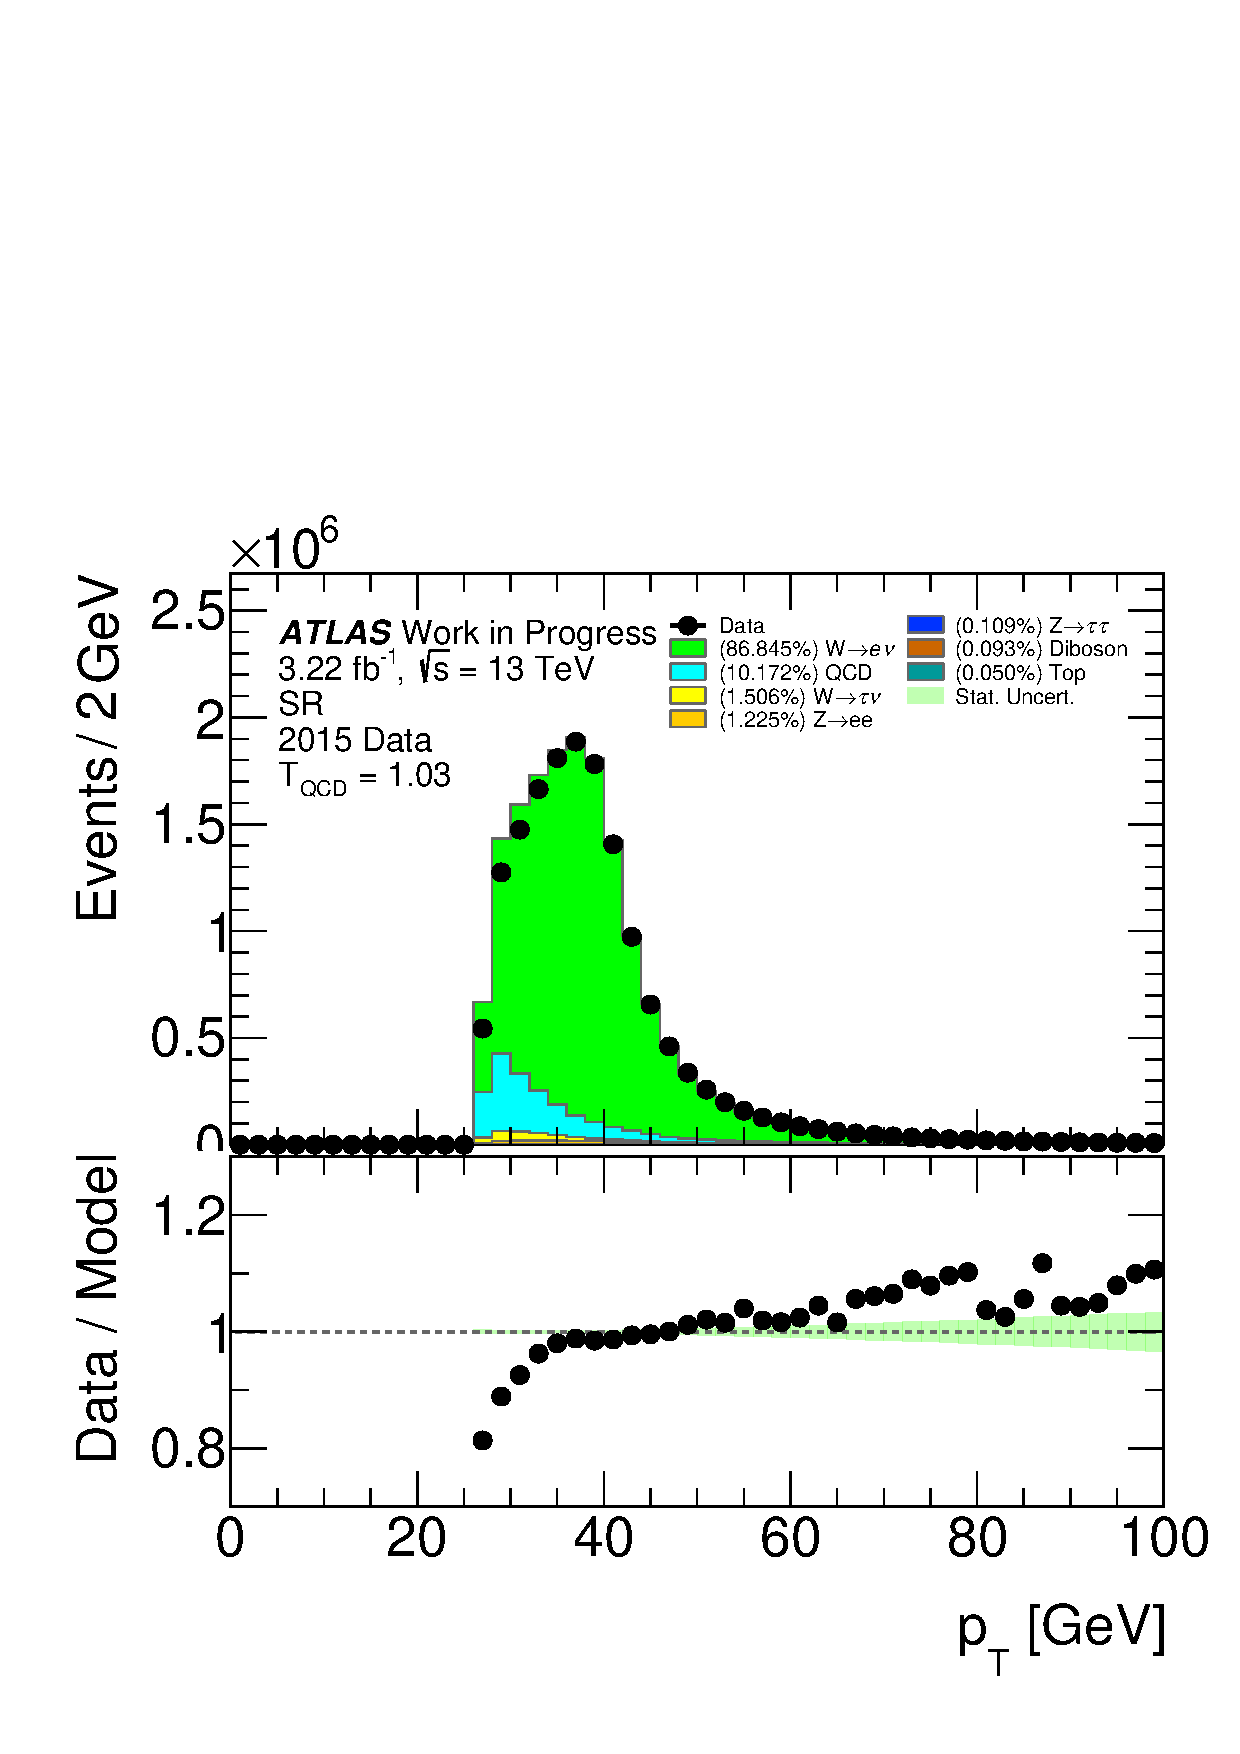
\includegraphics[width=0.45\textwidth]{figures/SR/dataMc-lep_0_pt-SR-bkgQCD-el.pdf}
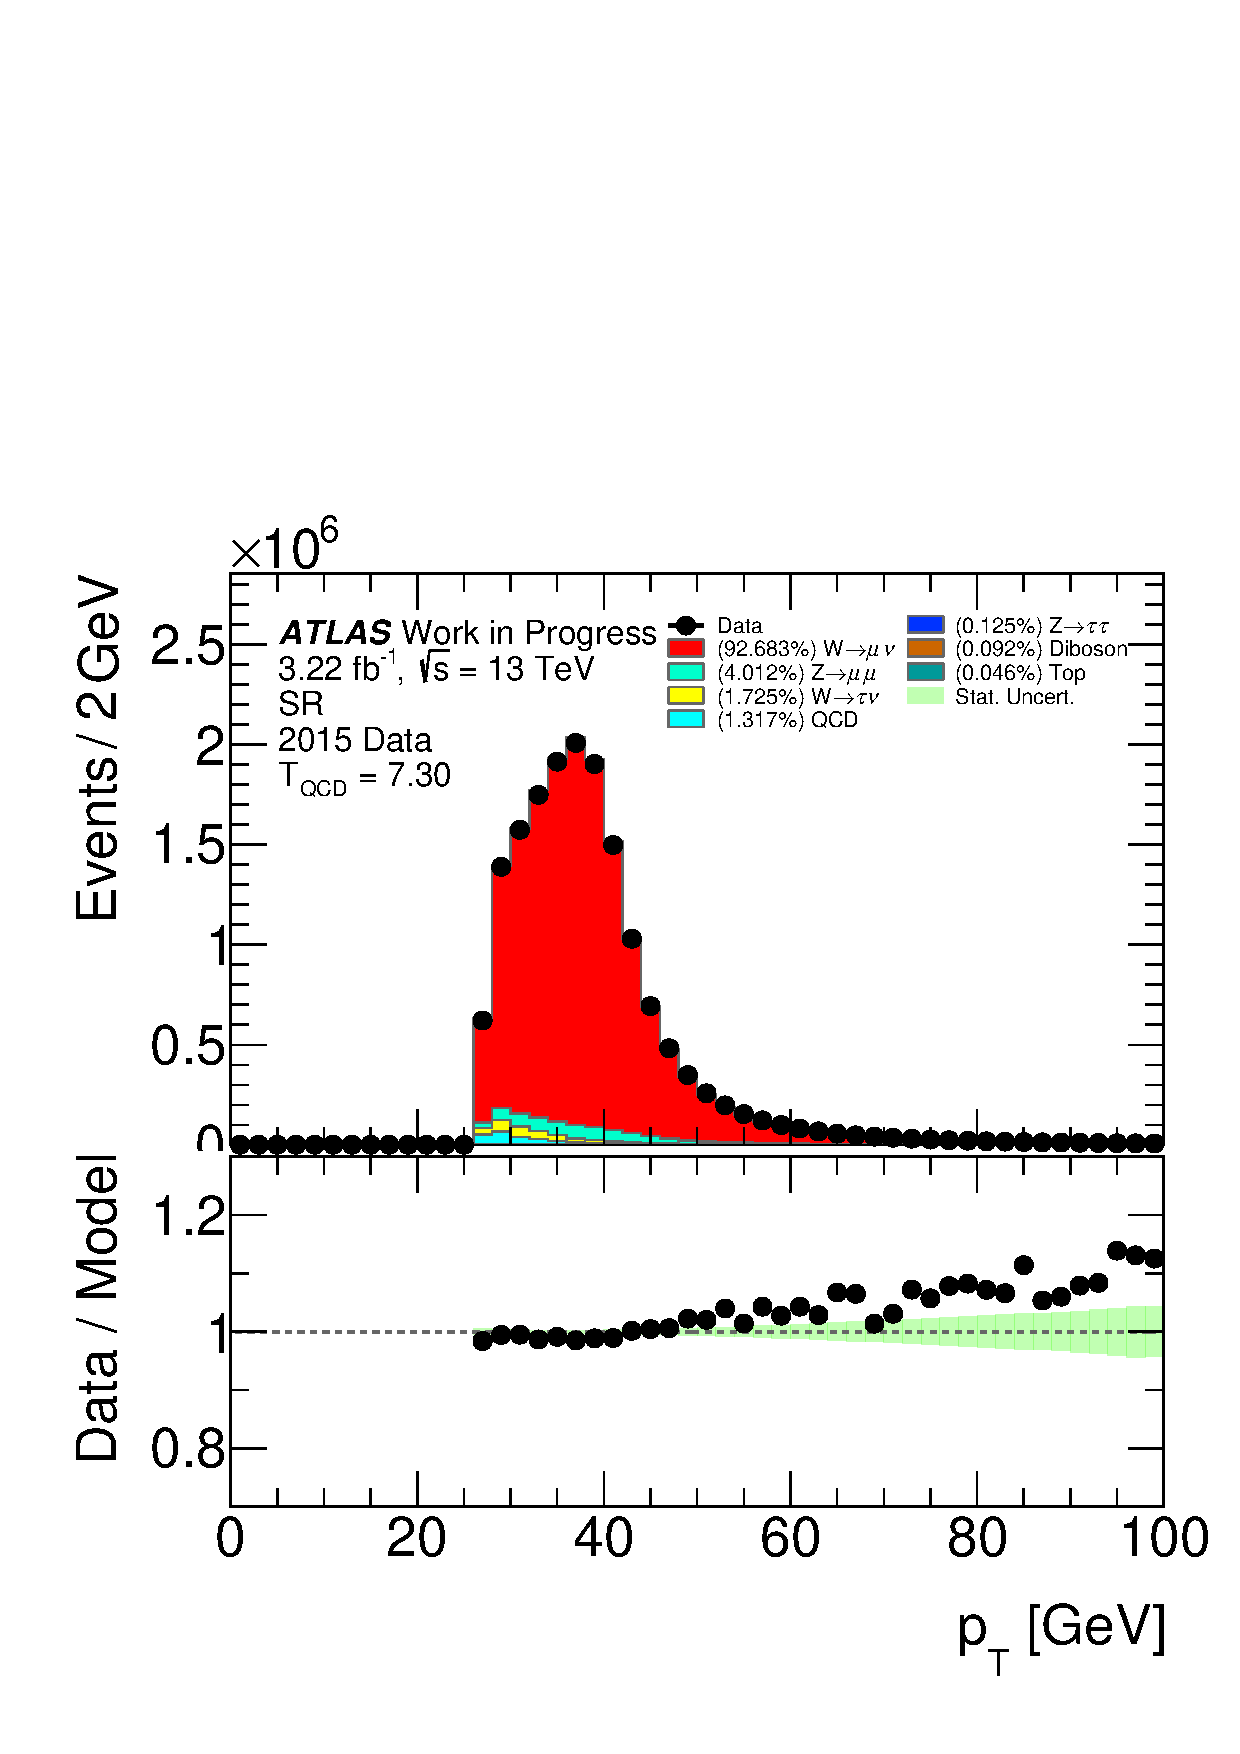
\includegraphics[width=0.45\textwidth]{figures/SR/dataMc-lep_0_pt-SR-bkgQCD-mu.pdf}
\caption{
Lepton transverse momentum distribution from the $W \rightarrow e\nu$ selection (left) and the $W \rightarrow \mu\nu$ selection (right). 
The expected contributions from all backgrounds are estimated with Monte Carlo simulations, except for the multijet background which is estimated with a data-driven method. 
% Systematic uncertainties for the signal and background distributions are combined in the shaded band, and 
Statistical uncertainties are shown on the data points.
Luminosity uncertainties are not included.
}
\label{fig:SR_lep_0_pt}
\end{figure}

\begin{figure}[htbp]
\centering
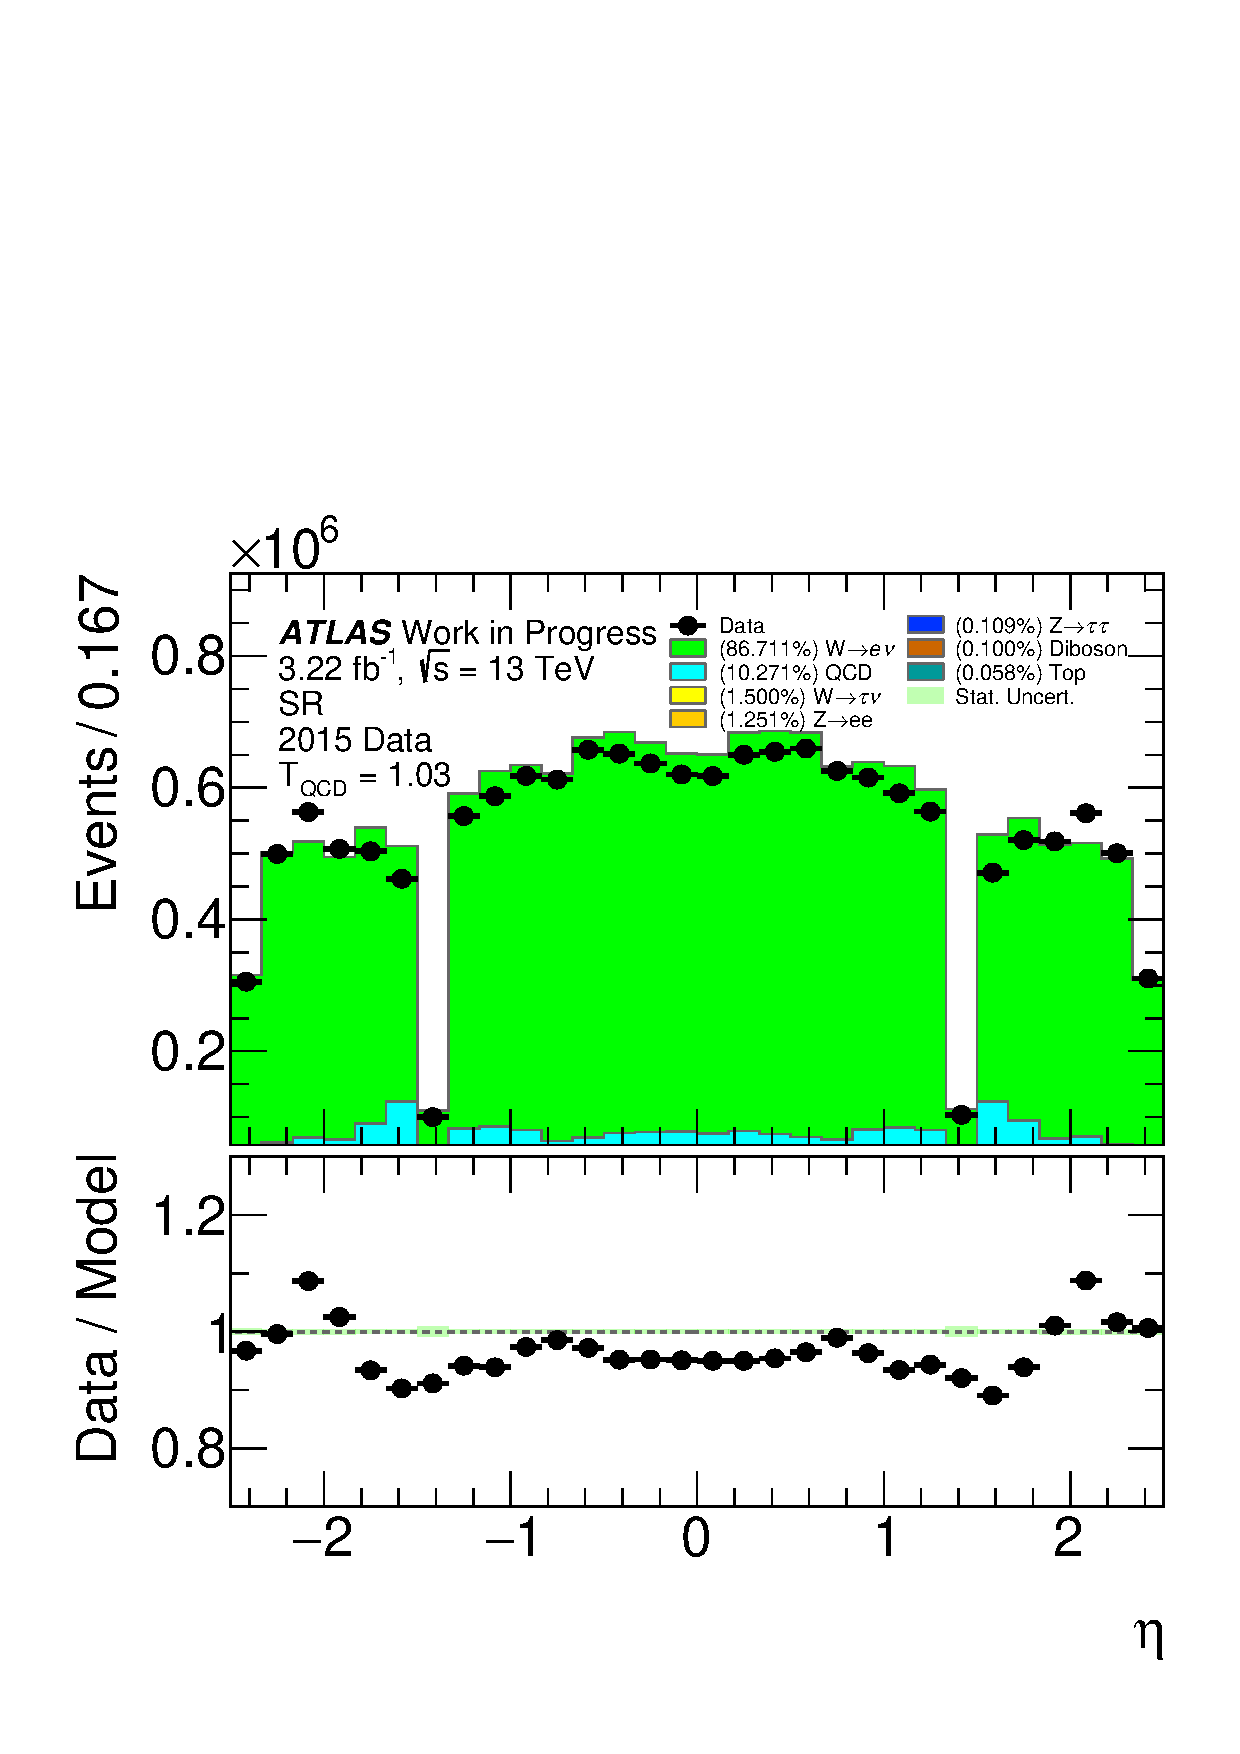
\includegraphics[width=0.45\textwidth]{figures/SR/dataMc-lep_0_eta-SR-bkgQCD-el.pdf}
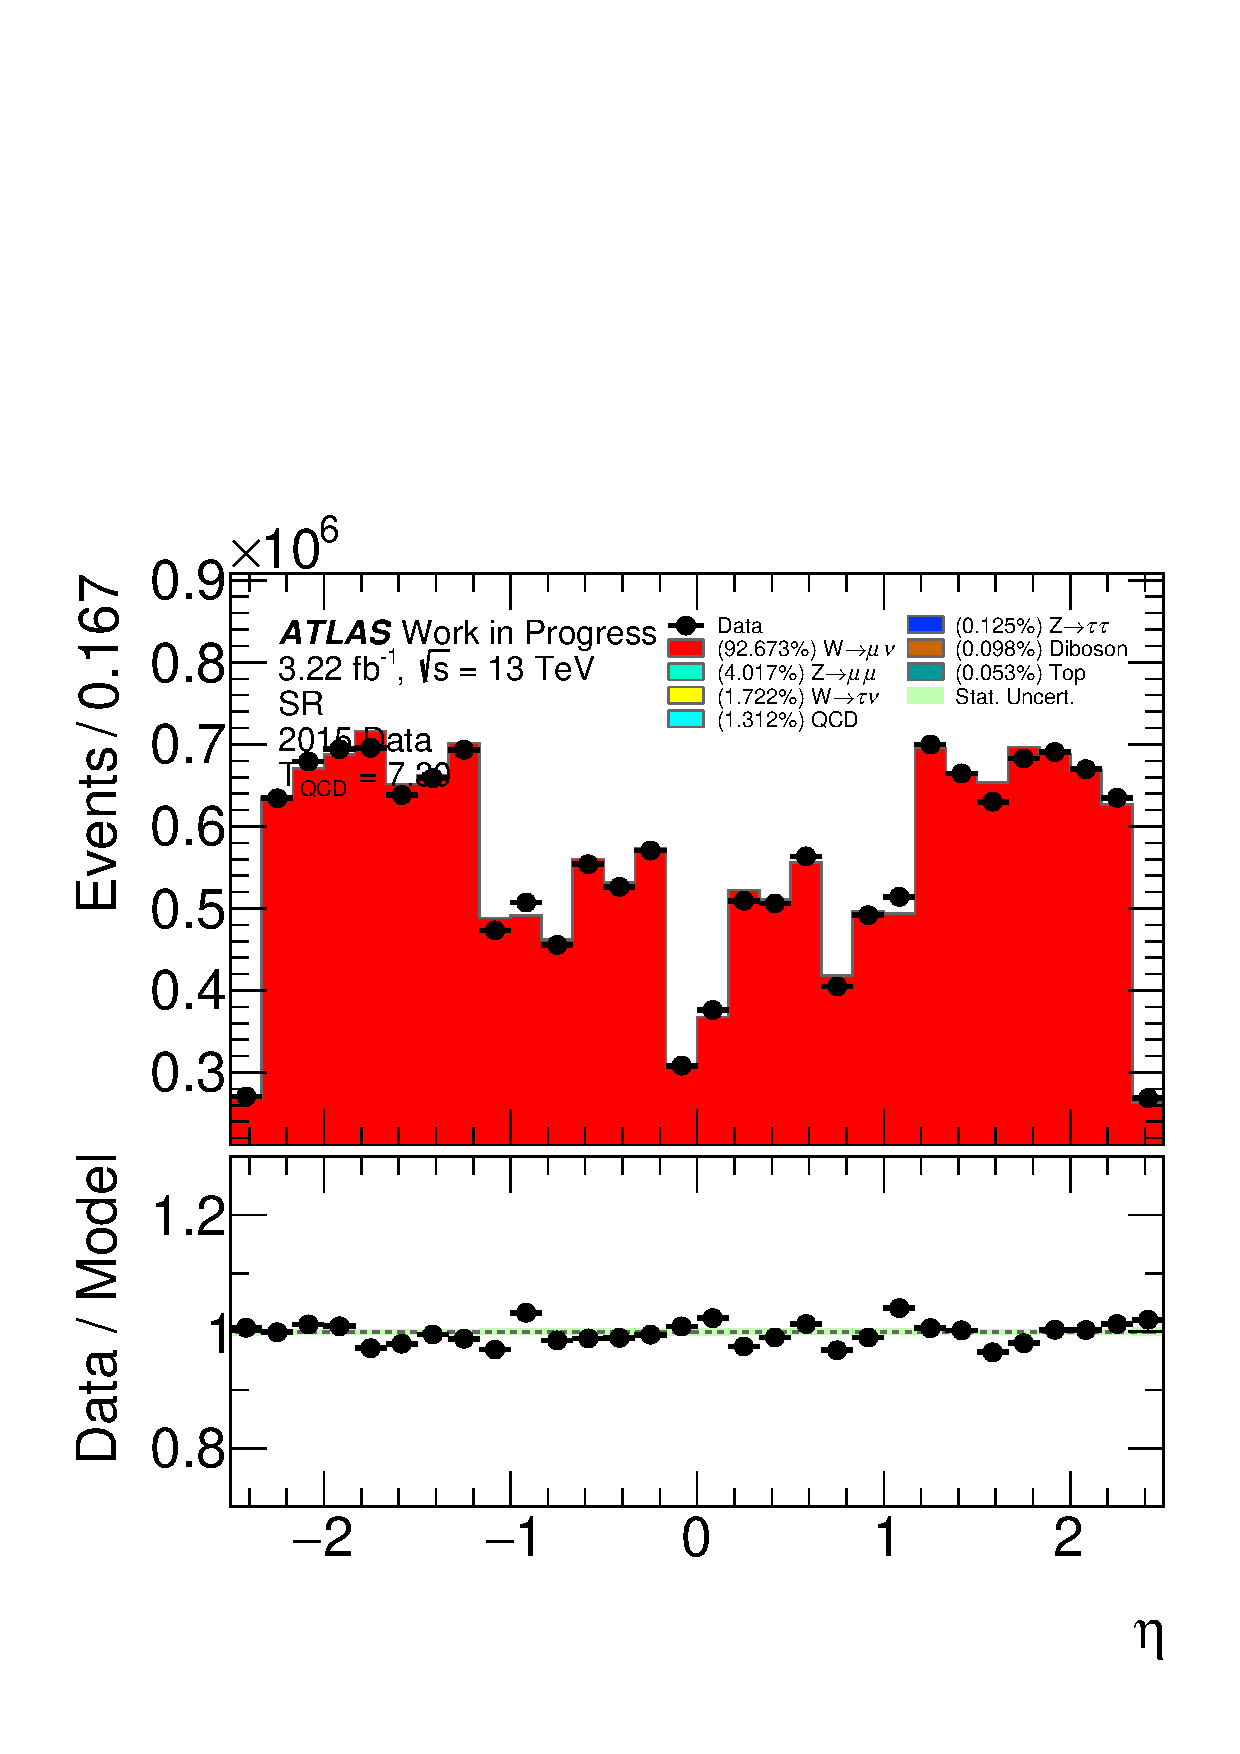
\includegraphics[width=0.45\textwidth]{figures/SR/dataMc-lep_0_eta-SR-bkgQCD-mu.pdf}
\caption{
Lepton  pseudorapidity distribution from the $W \rightarrow e\nu$ selection (left) and the $W \rightarrow \mu\nu$ selection (right). 
The expected contributions from all backgrounds are estimated with Monte Carlo simulations, except for the multijet background which is estimated with a data-driven method. 
% Systematic uncertainties for the signal and background distributions are combined in the shaded band, and 
Statistical uncertainties are shown on the data points.
Luminosity uncertainties are not included.
}
\label{fig:SR_lep_0_eta}
\end{figure}

\begin{figure}[htbp]
\centering
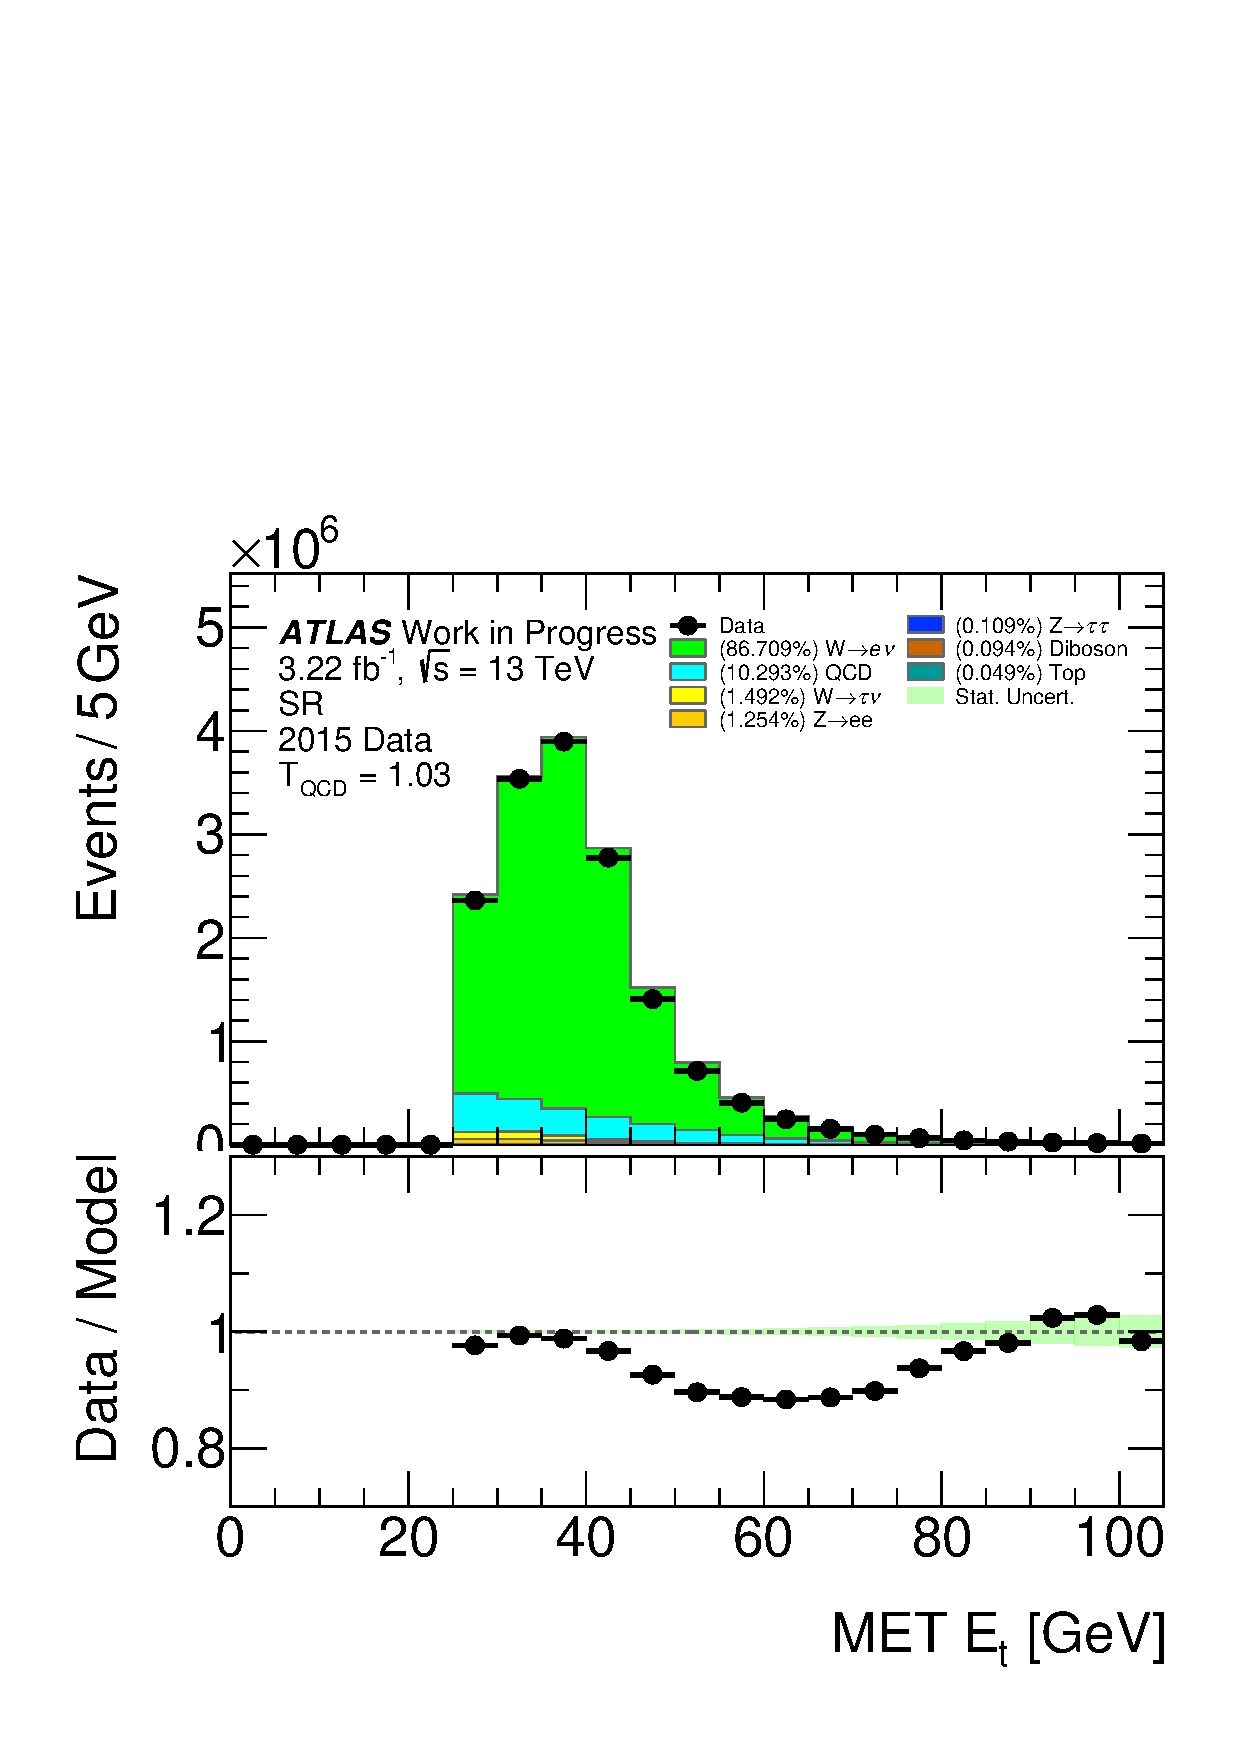
\includegraphics[width=0.45\textwidth]{figures/SR/dataMc-met_reco_et-SR-bkgQCD-el.pdf}
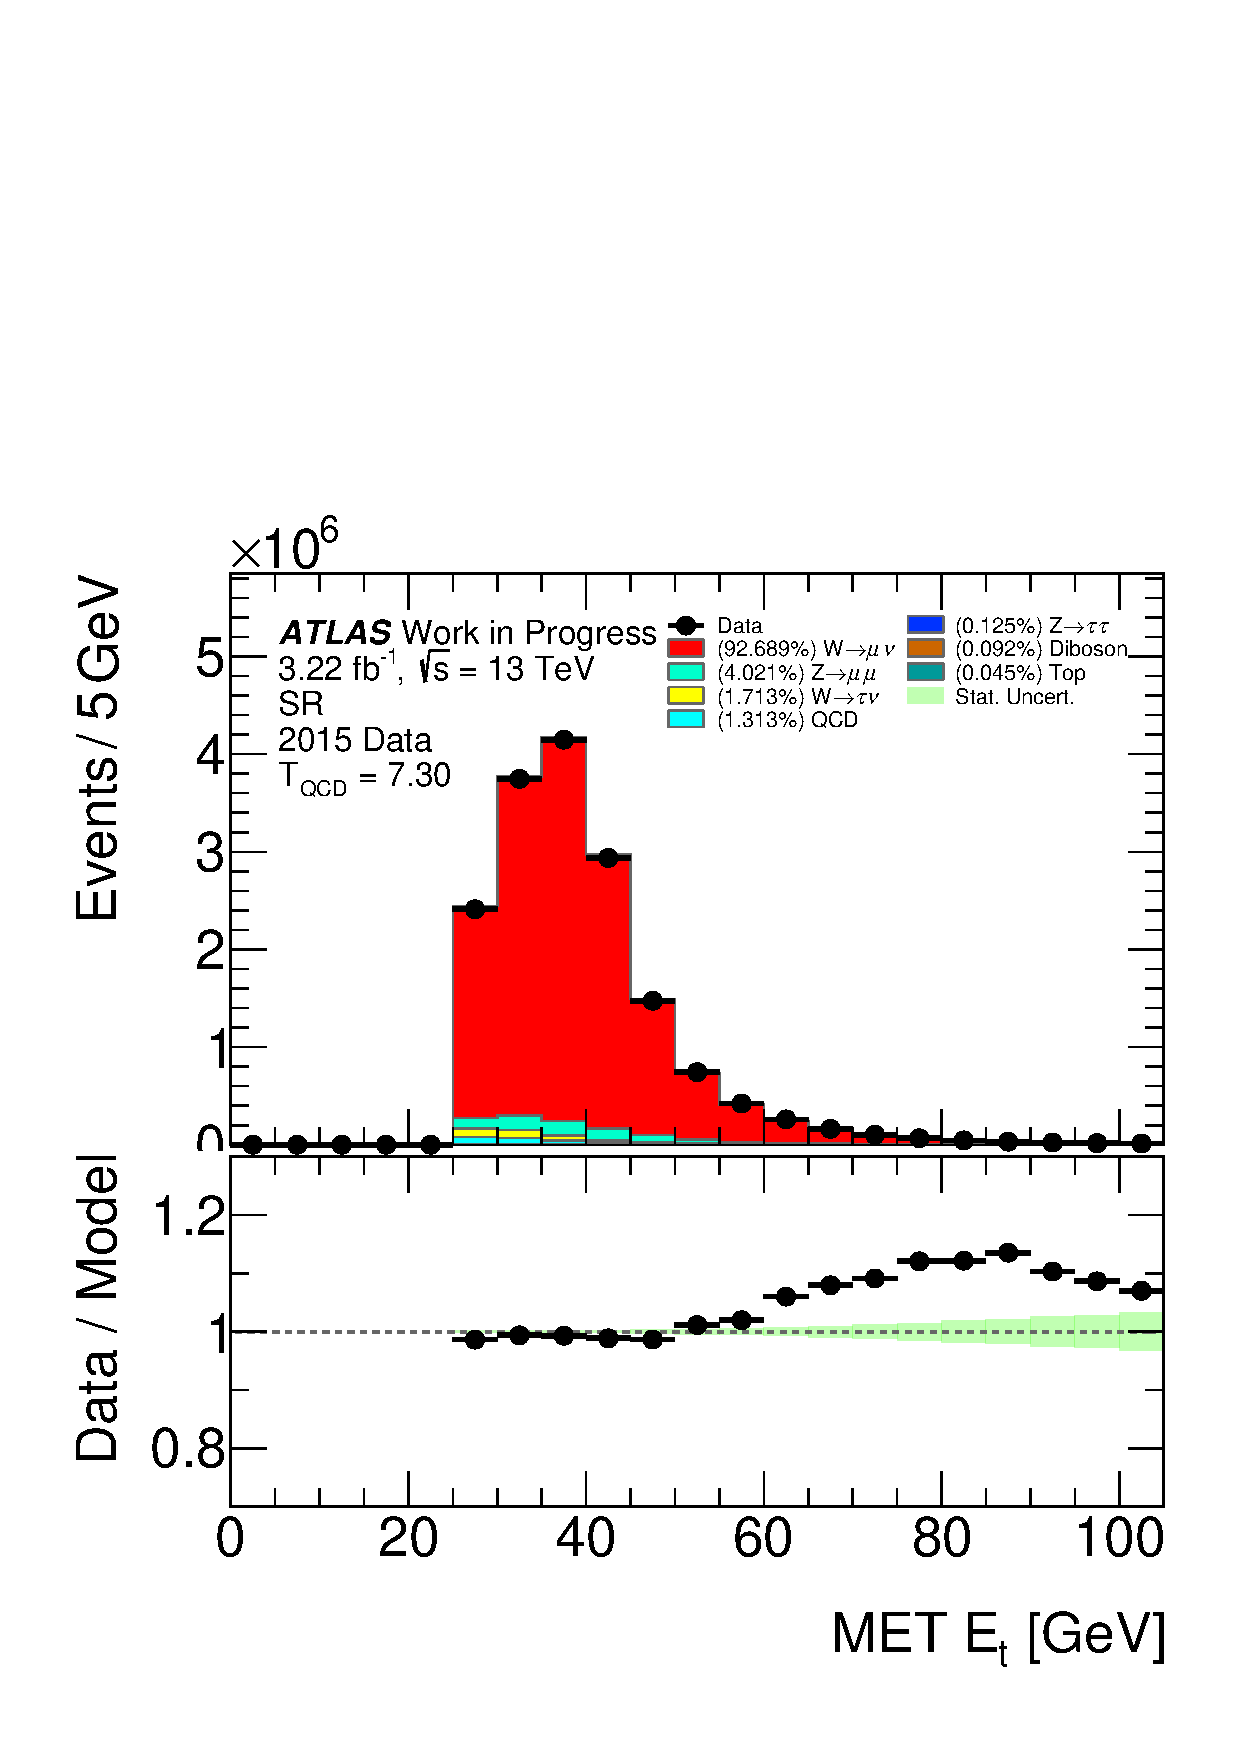
\includegraphics[width=0.45\textwidth]{figures/SR/dataMc-met_reco_et-SR-bkgQCD-mu.pdf}
\caption{
Missing transverse energy distribution from the $W \rightarrow e\nu$ selection (left) and the $W \rightarrow \mu\nu$ selection (right).
The $E_{T}^{miss}$ has been recalibrated using the best energy calibration for each of the identified physics objects.
The expected contributions from all backgrounds are estimated with Monte Carlo simulations, except for the multijet background which is estimated with a data-driven method. 
% Systematic uncertainties for the signal and background distributions are combined in the shaded band, and 
Statistical uncertainties are shown on the data points.
Luminosity uncertainties are not included.
}
\label{fig:SR_met_reco_et}
\end{figure}

\begin{figure}[htbp]
\centering
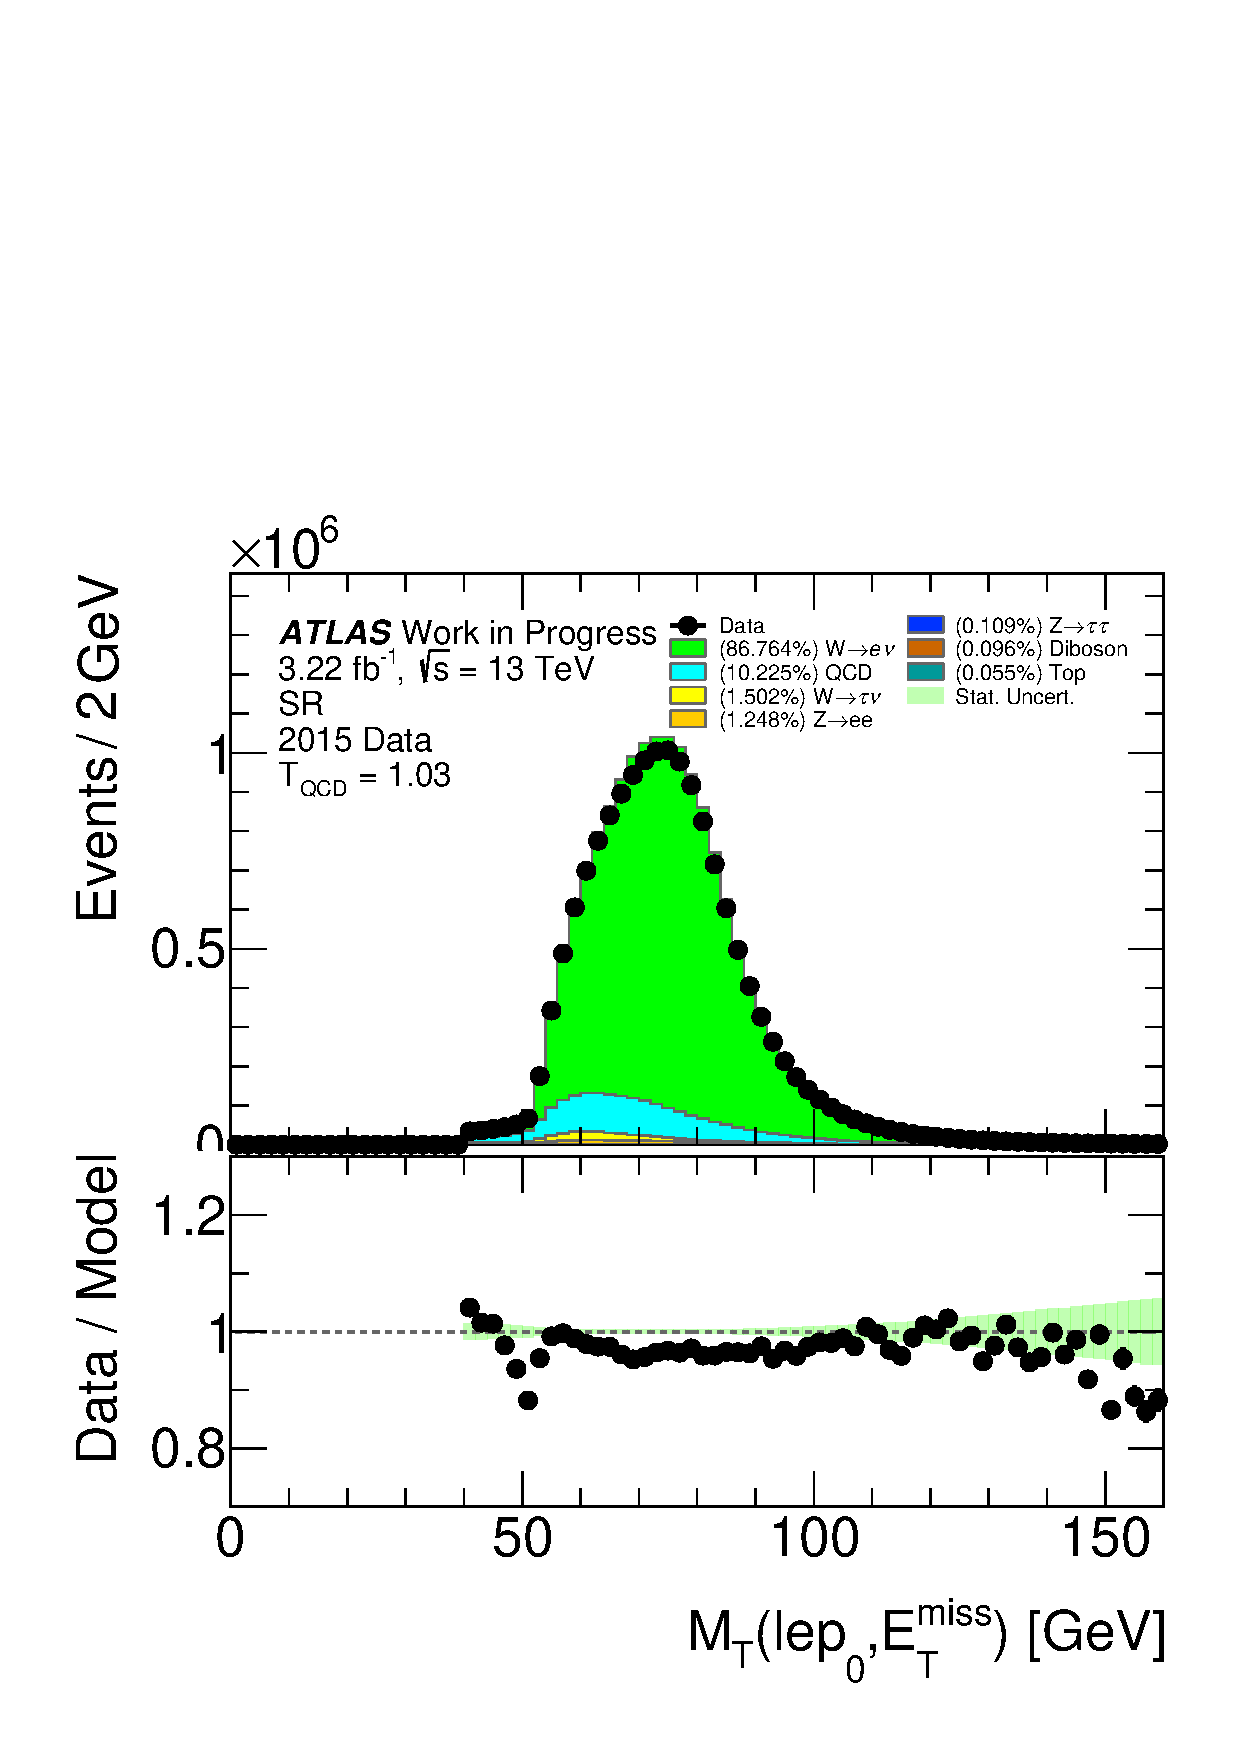
\includegraphics[width=0.45\textwidth]{figures/SR/dataMc-lepmet_mt-SR-bkgQCD-el.pdf}
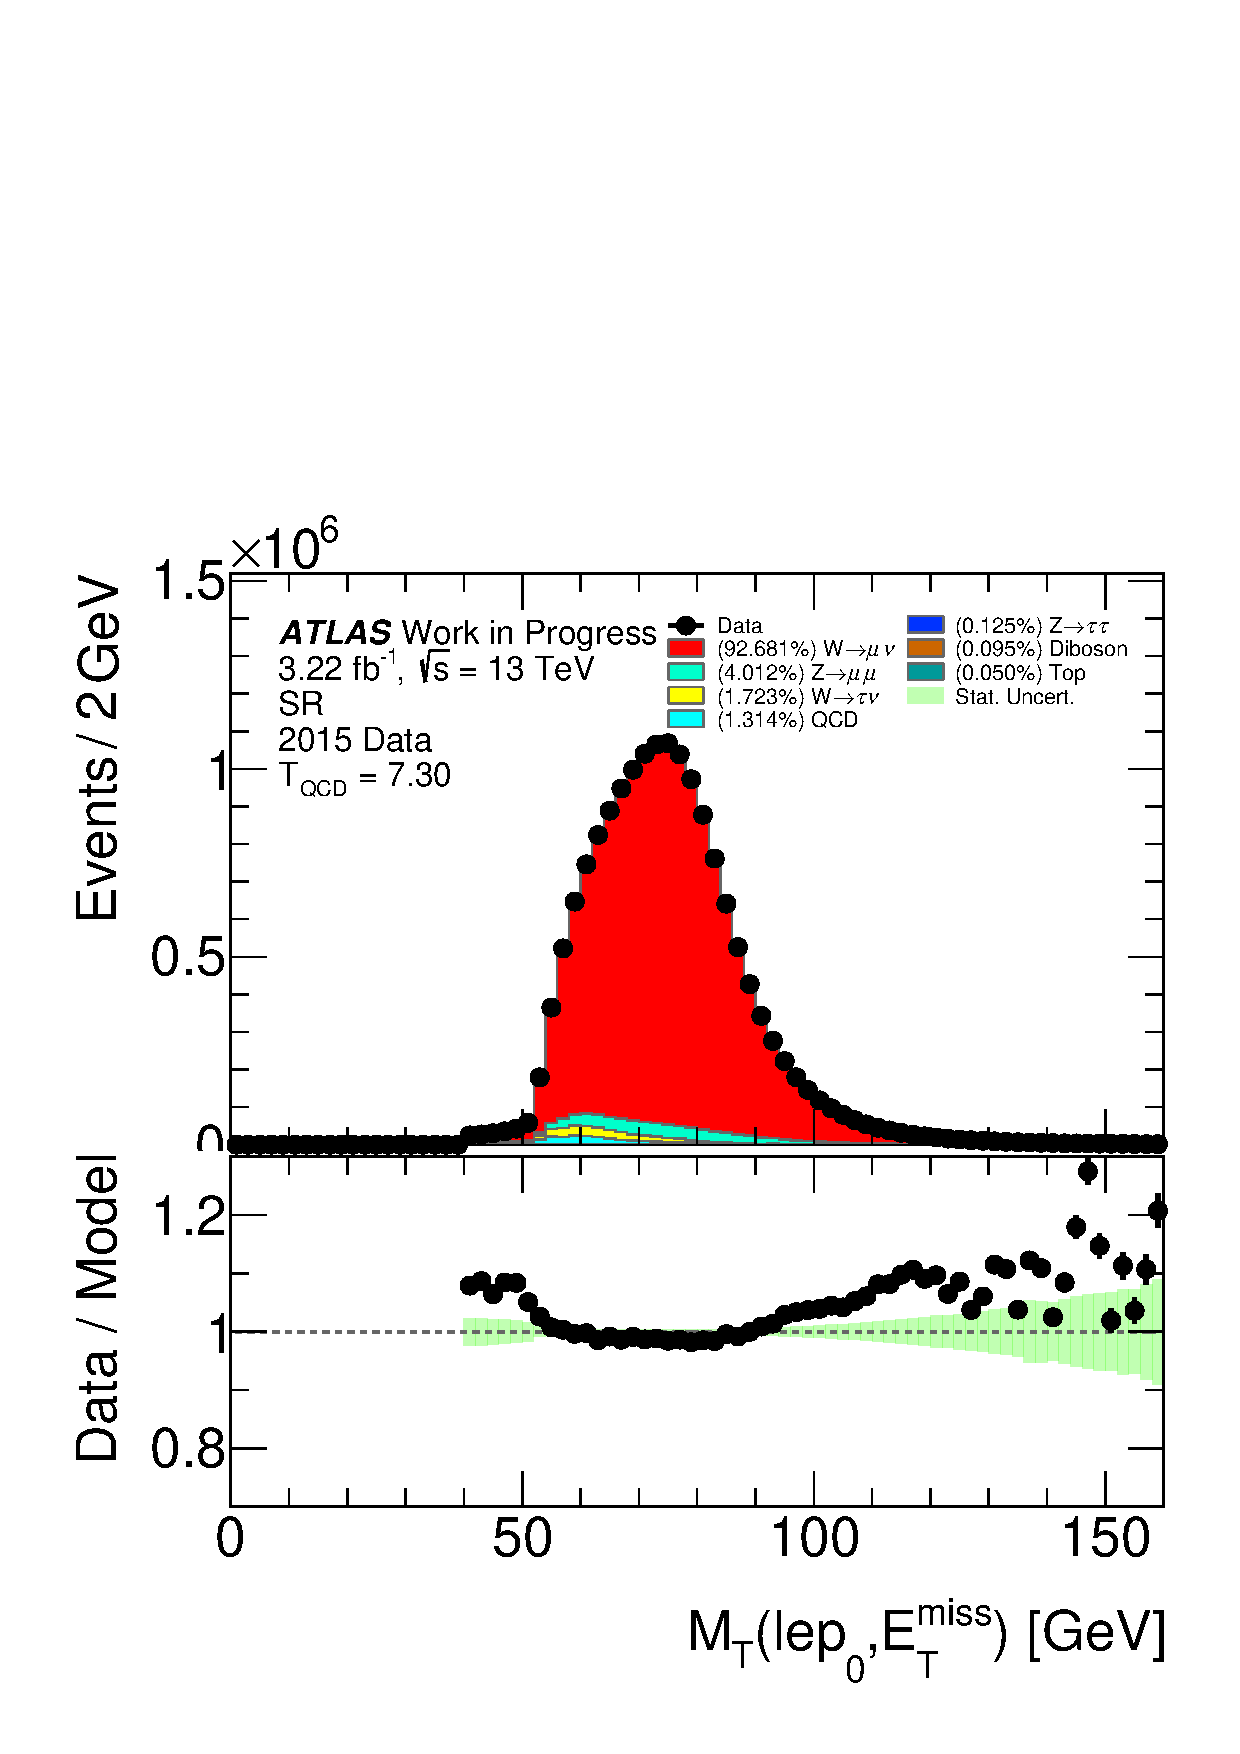
\includegraphics[width=0.45\textwidth]{figures/SR/dataMc-lepmet_mt-SR-bkgQCD-mu.pdf}
\caption{
Transverse mass distribution, calculated from the lepton and the $E_{T}^{miss}$ from the $W \rightarrow e\nu$ selection (left) and the $W \rightarrow \mu\nu$ selection (right).
The $E_{T}^{miss}$ has been recalibrated using the best energy calibration for each of the identified physics objects.
The expected contributions from all backgrounds are estimated with Monte Carlo simulations, except for the multijet background which is estimated with a data-driven method. 
% Systematic uncertainties for the signal and background distributions are combined in the shaded band, and 
Statistical uncertainties are shown on the data points.
Luminosity uncertainties are not included.
}
\label{fig:SR_met_reco_et}
\end{figure}

\begin{figure}[htbp]
\centering
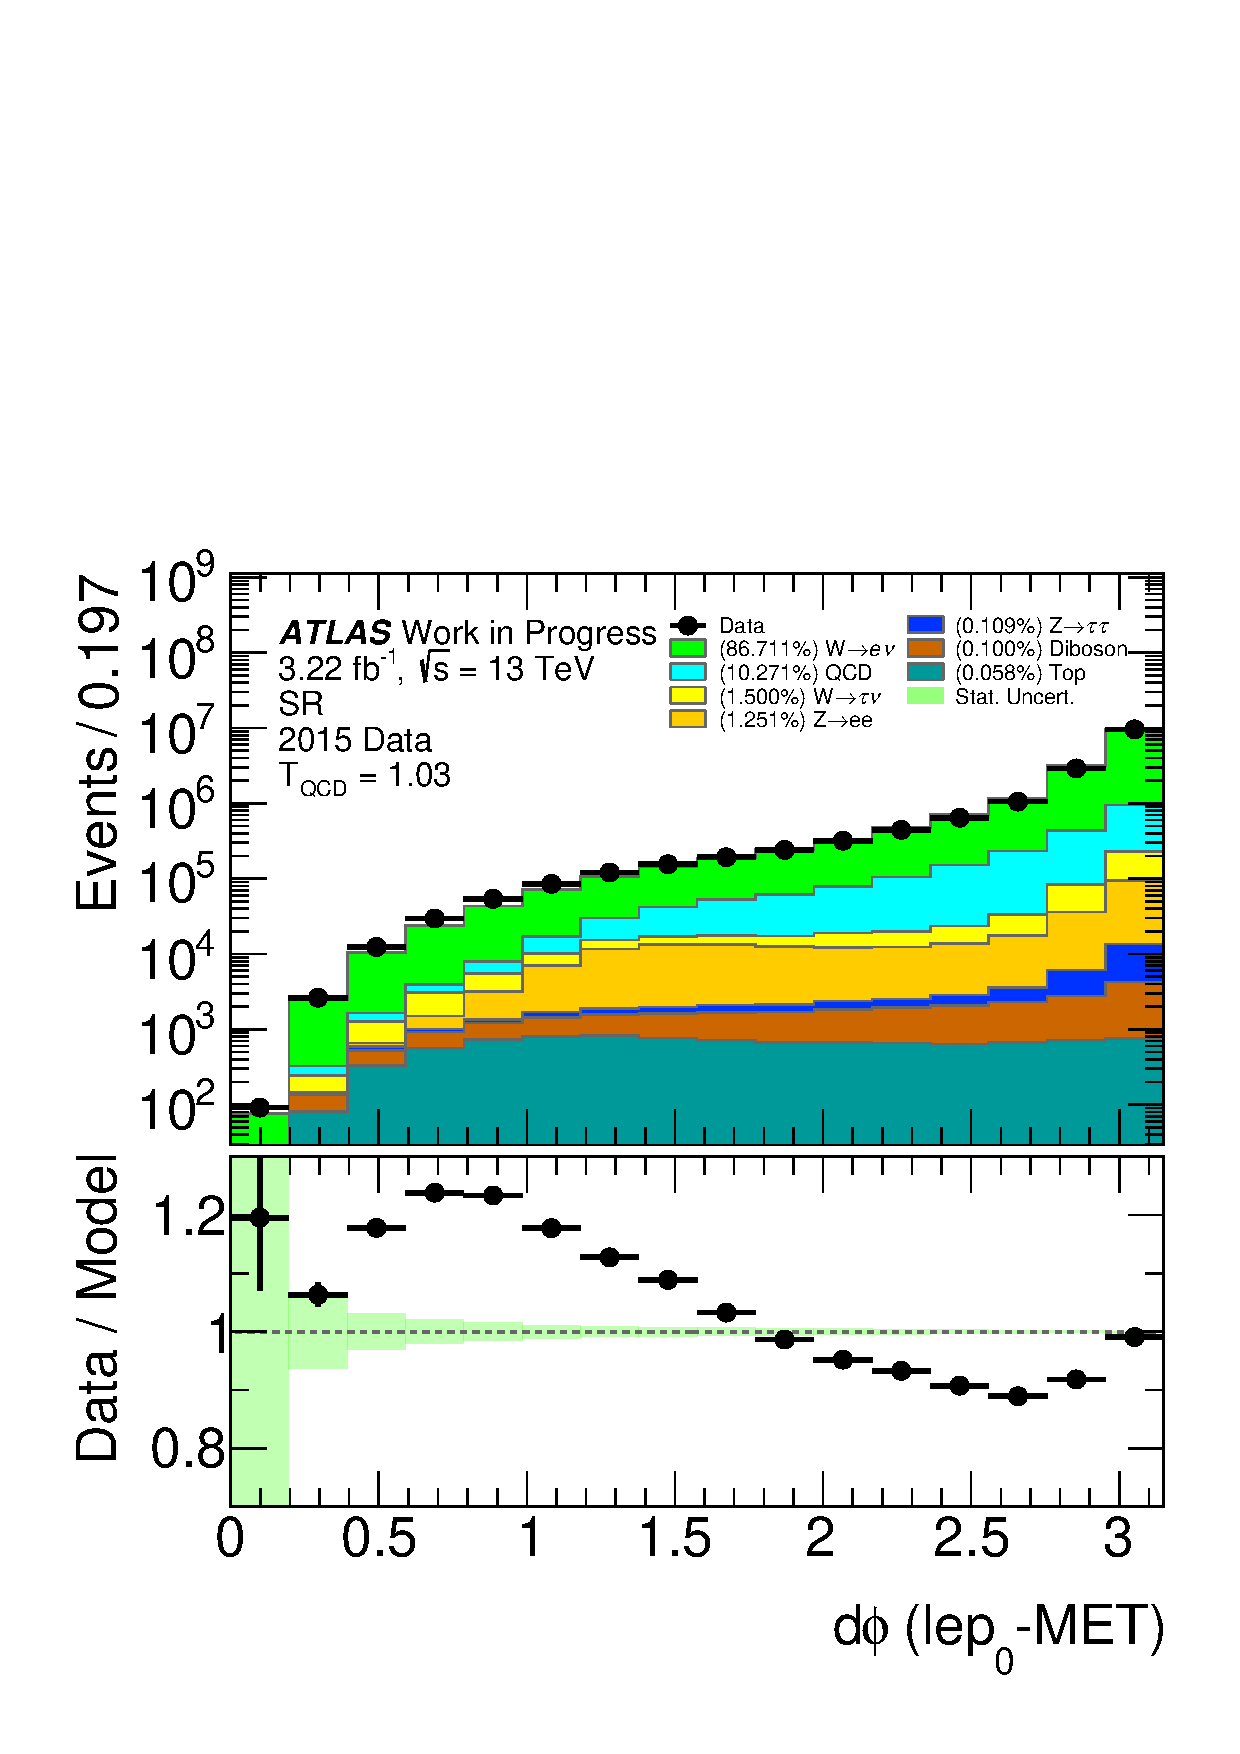
\includegraphics[width=0.45\textwidth]{figures/SR/dataMc-lepmet_dphi-SR-bkgQCD-el-log.pdf}
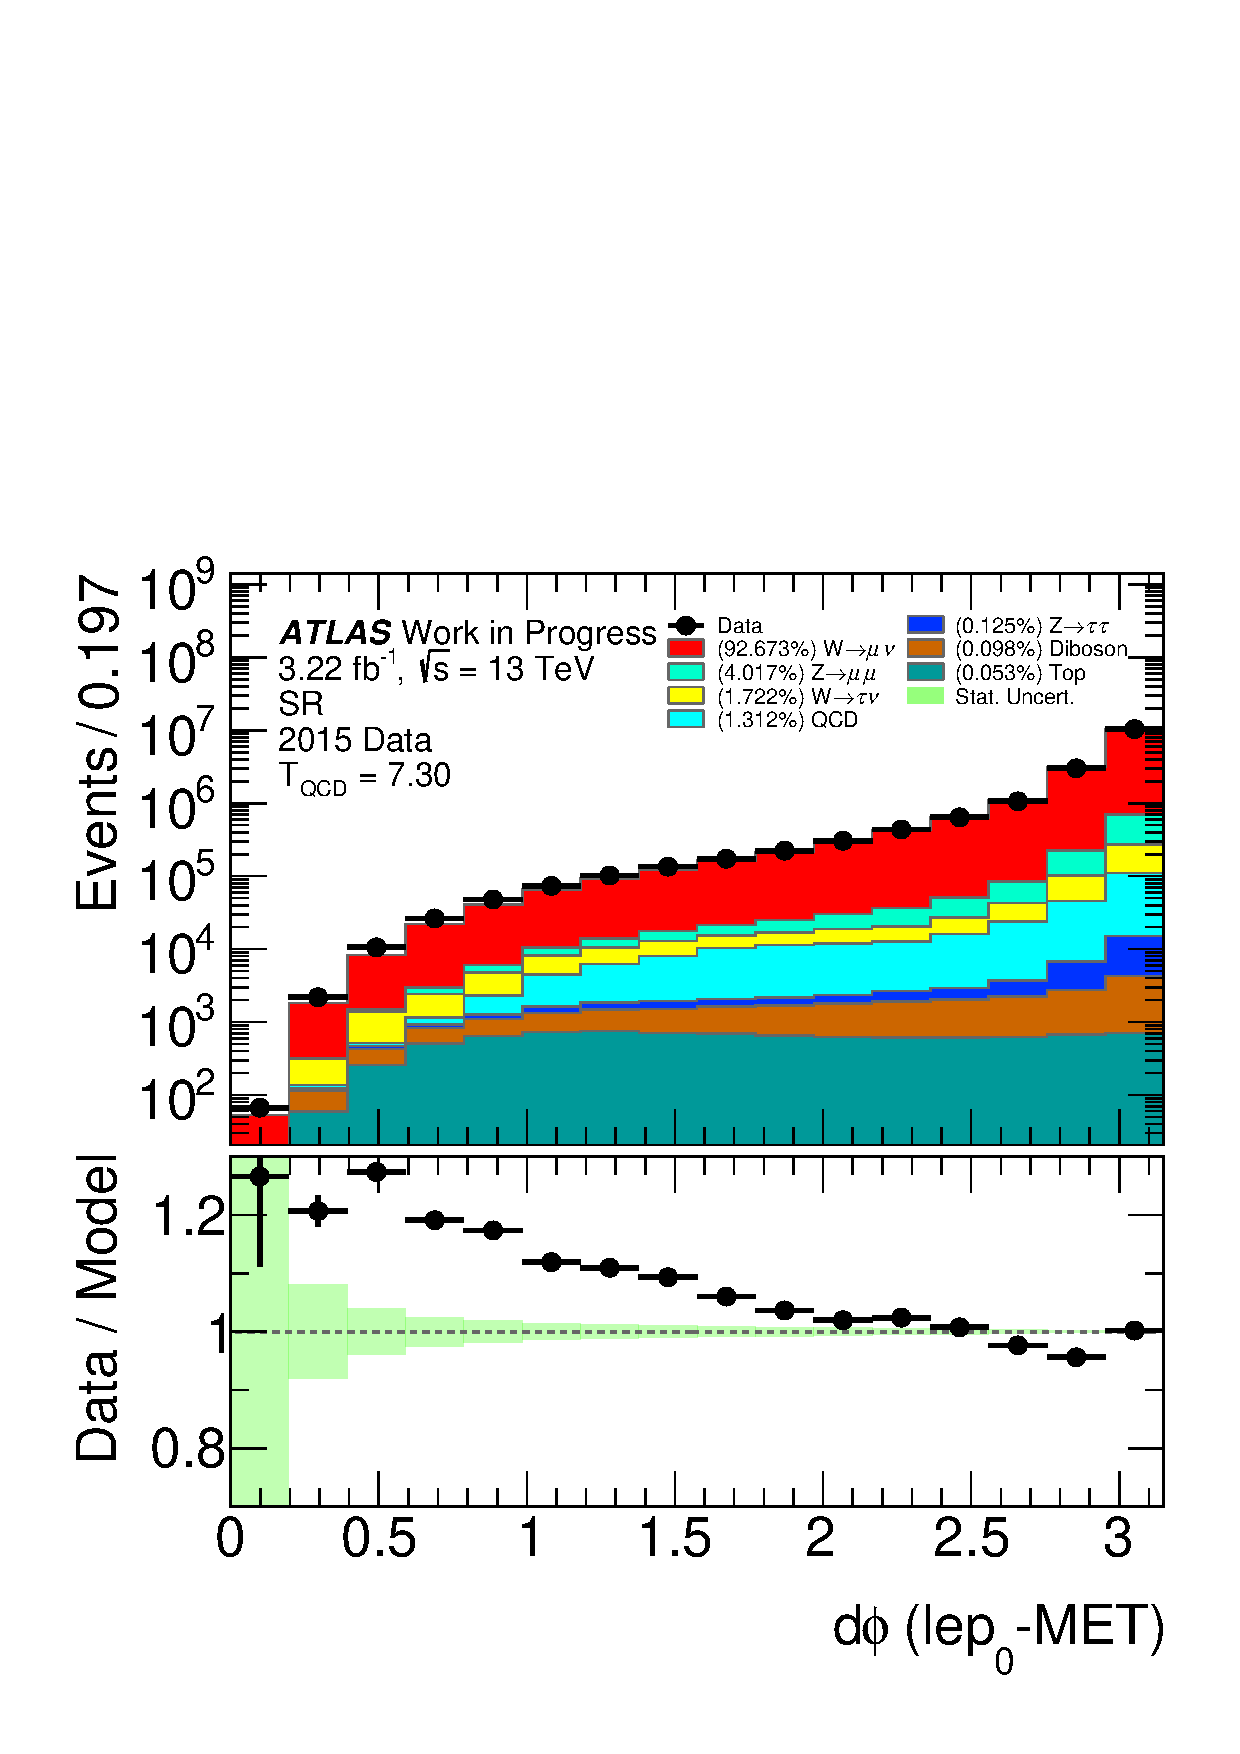
\includegraphics[width=0.45\textwidth]{figures/SR/dataMc-lepmet_dphi-SR-bkgQCD-mu-log.pdf}
\caption{
Azimuthal angle distribution, calculated as azimuthal angle difference of the leading lepton and the $E_{T}^{miss}$ from the $W \rightarrow e\nu$ selection (left) and the $W \rightarrow \mu\nu$ selection (right).
The $E_{T}^{miss}$ has been recalibrated using the best energy calibration for each of the identified physics objects.
The expected contributions from all backgrounds are estimated with Monte Carlo simulations, except for the multijet background which is estimated with a data-driven method. 
% Systematic uncertainties for the signal and background distributions are combined in the shaded band, and 
Statistical uncertainties are shown on the data points.
Luminosity uncertainties are not included.
}
\label{fig:SR_lepmet_dphi}
\end{figure}

% ##################
% ZR
% ##################

\begin{figure}[htbp]
\centering
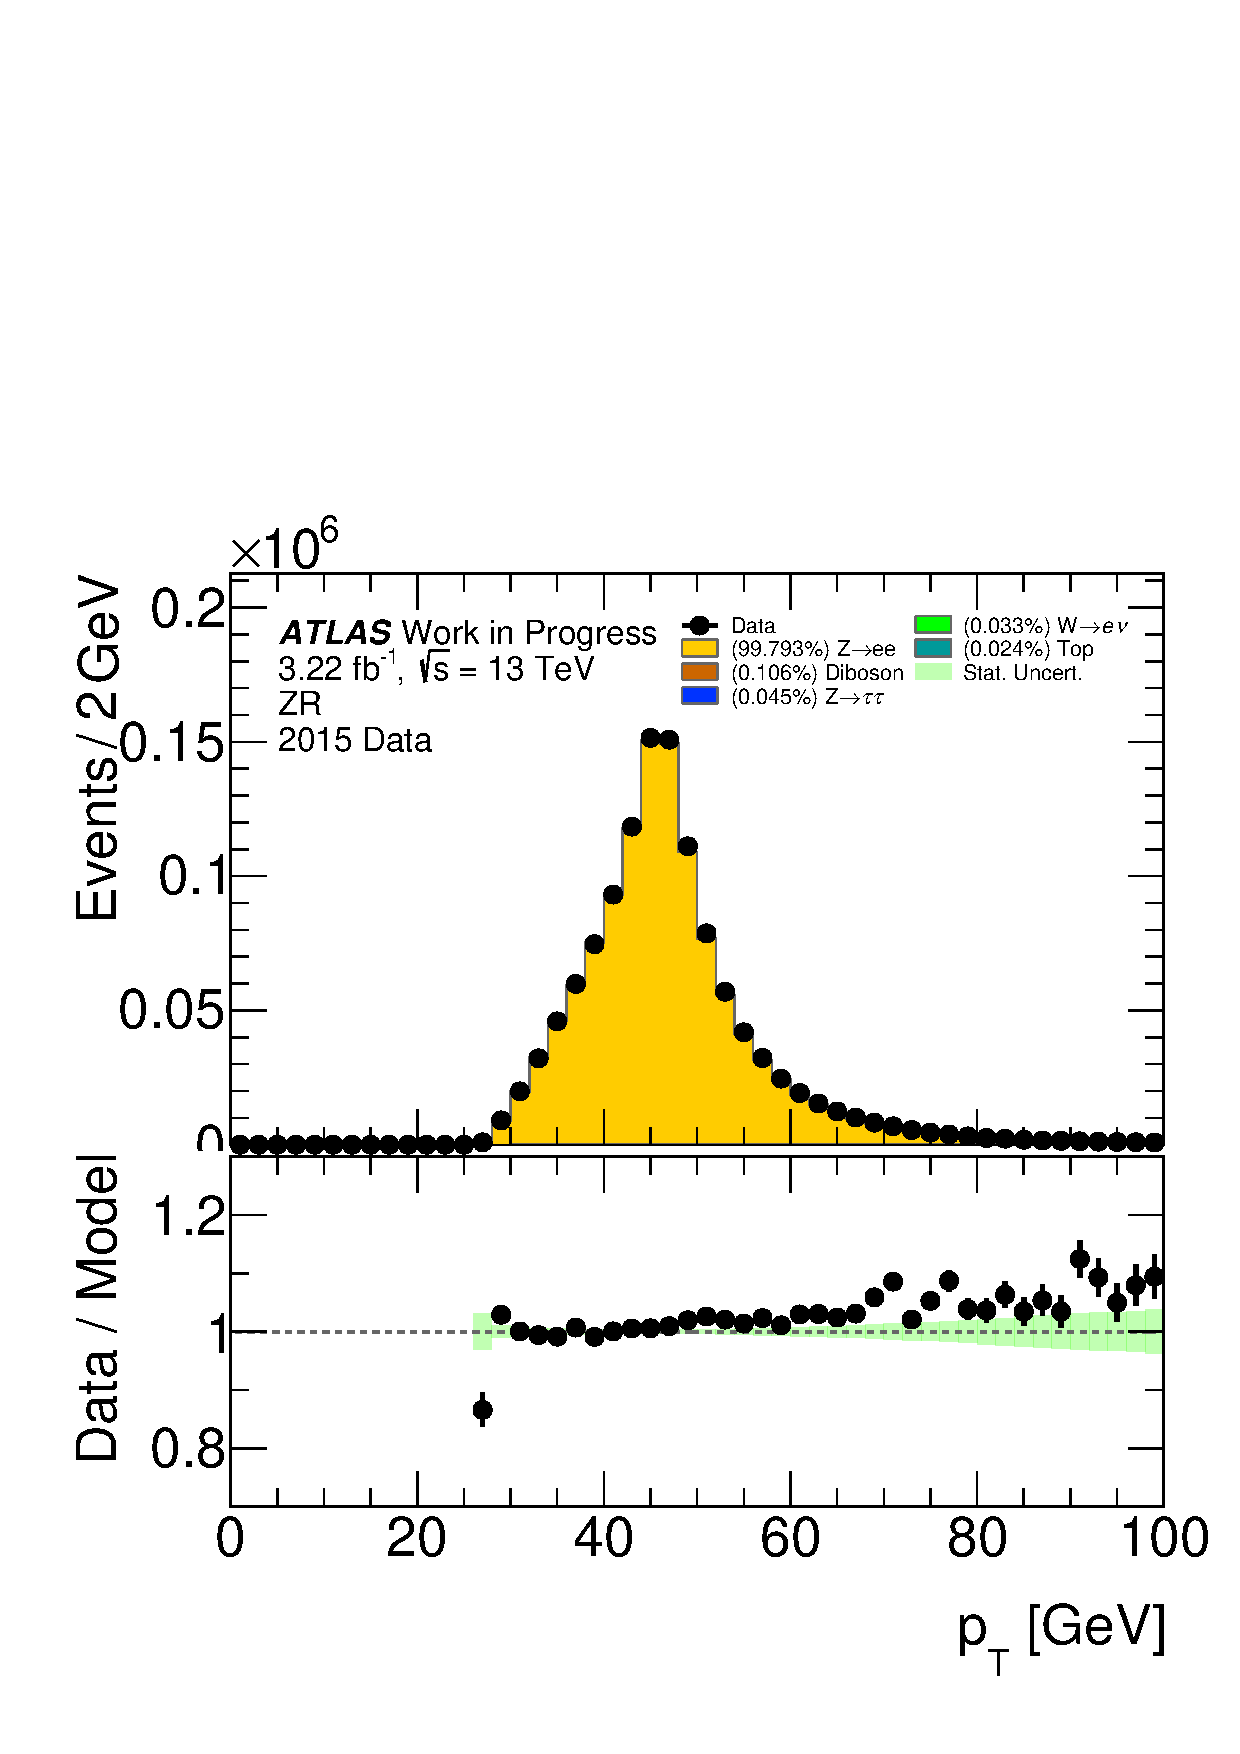
\includegraphics[width=0.45\textwidth]{figures/ZR/dataMc-lep_0_pt-ZR-el.pdf}
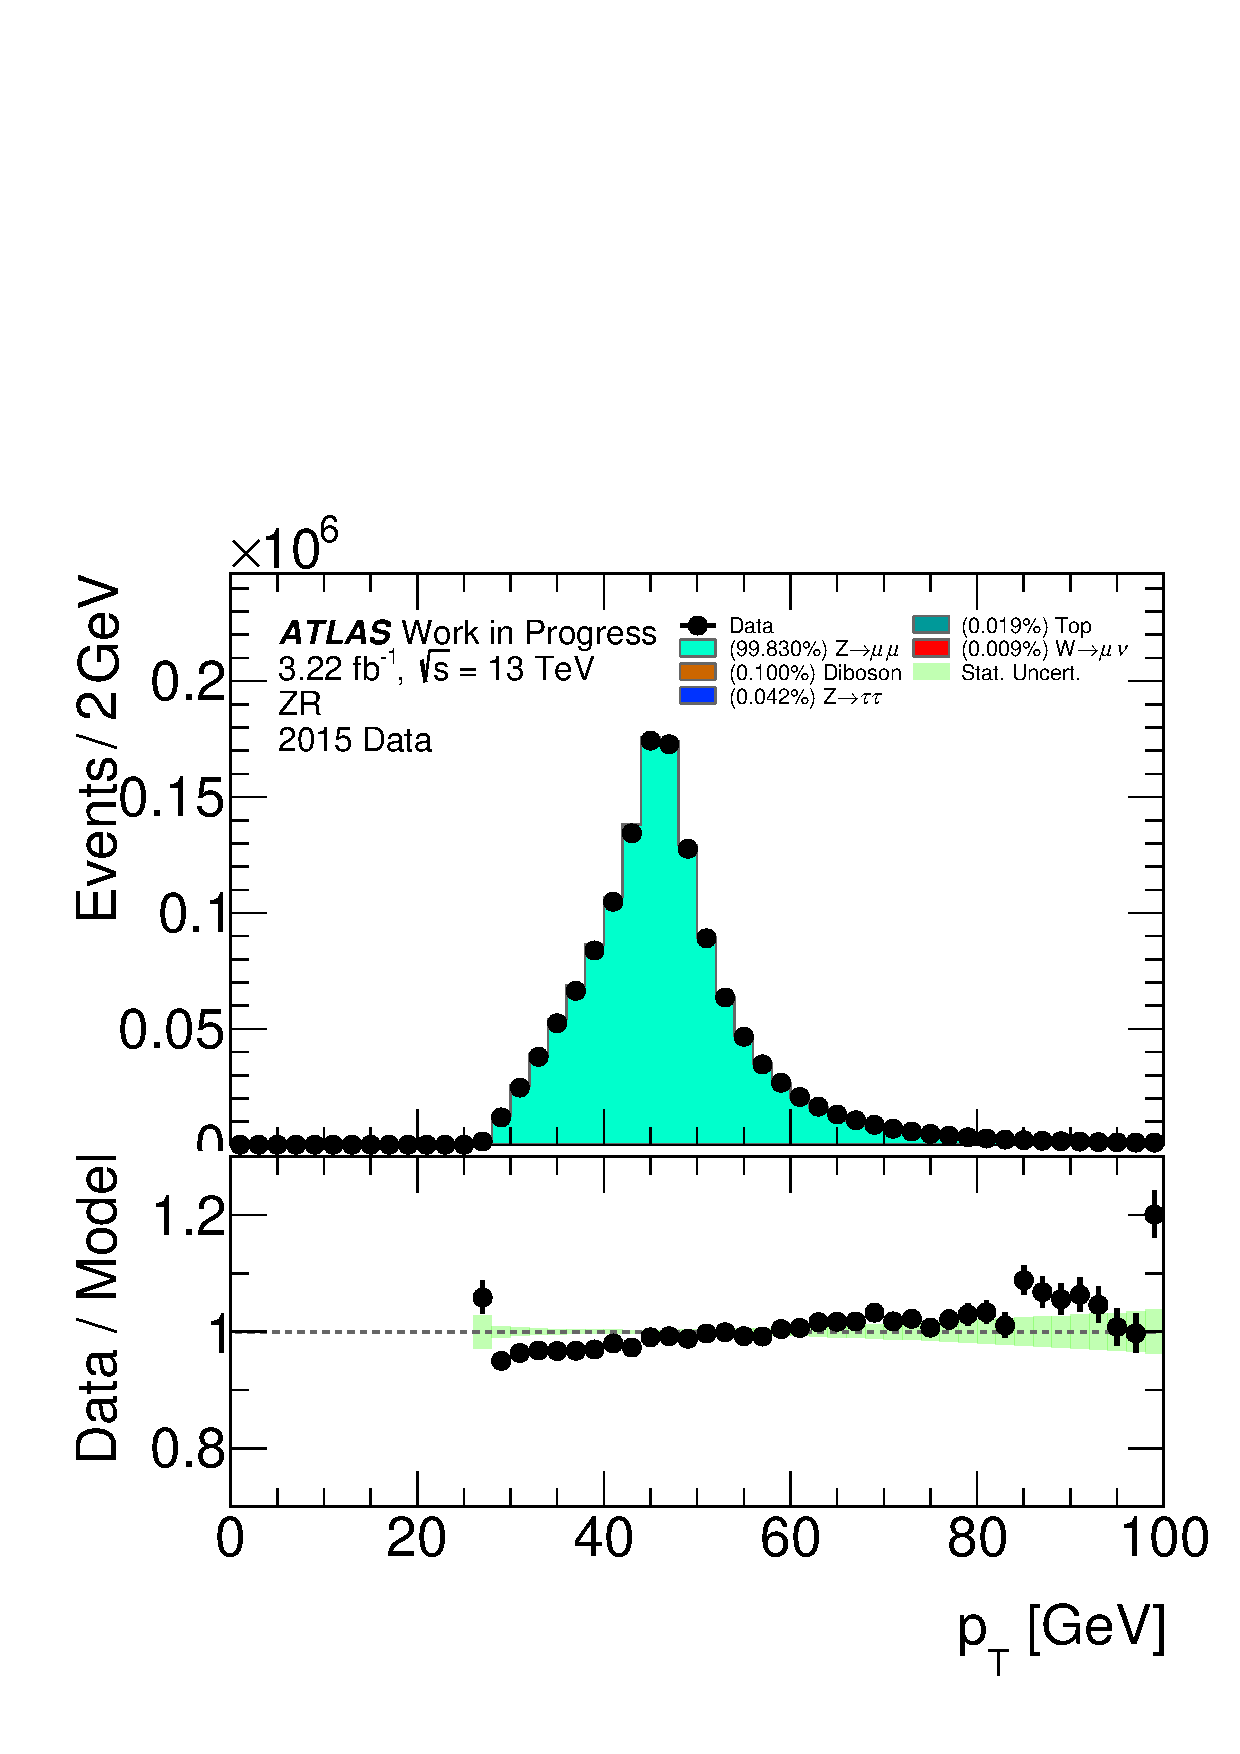
\includegraphics[width=0.45\textwidth]{figures/ZR/dataMc-lep_0_pt-ZR-mu.pdf}
\caption{
Leading lepton transverse momentum distributions from the $Z \rightarrow e^+e^-$ selection (left) and the $Z \rightarrow \mu^+\mu^-$  selection (right).
The expected contributions from all backgrounds are estimated with Monte Carlo simulations.
The background processes are heavily suppressed and not visible on the linear scale. 
% Systematic uncertainties for the signal and background distributions are combined in the shaded band, and 
Statistical uncertainties are shown on the data points.
Luminosity uncertainties are not included.
}
\label{fig:ZR_lep_0_pt}
\end{figure}

\begin{figure}[htbp]
\centering
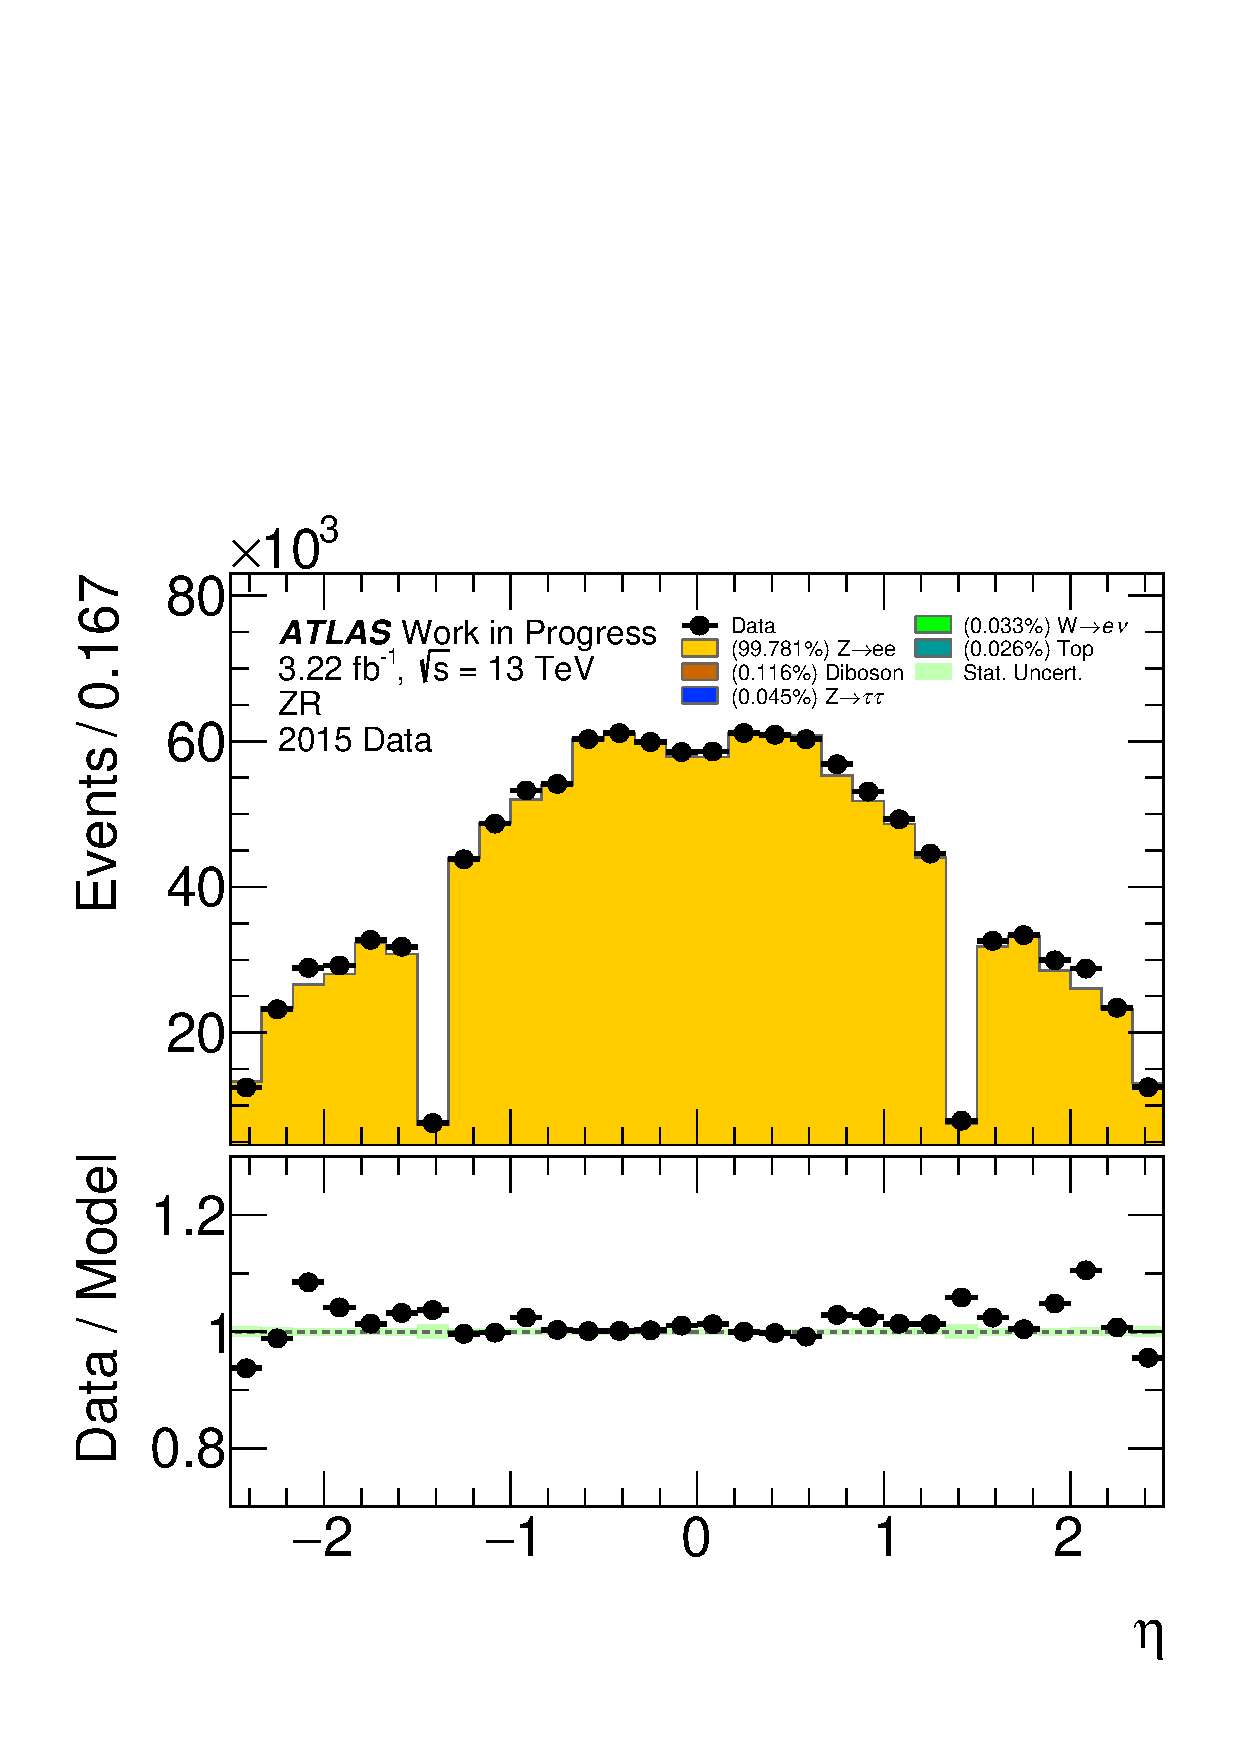
\includegraphics[width=0.45\textwidth]{figures/ZR/dataMc-lep_0_eta-ZR-el.pdf}
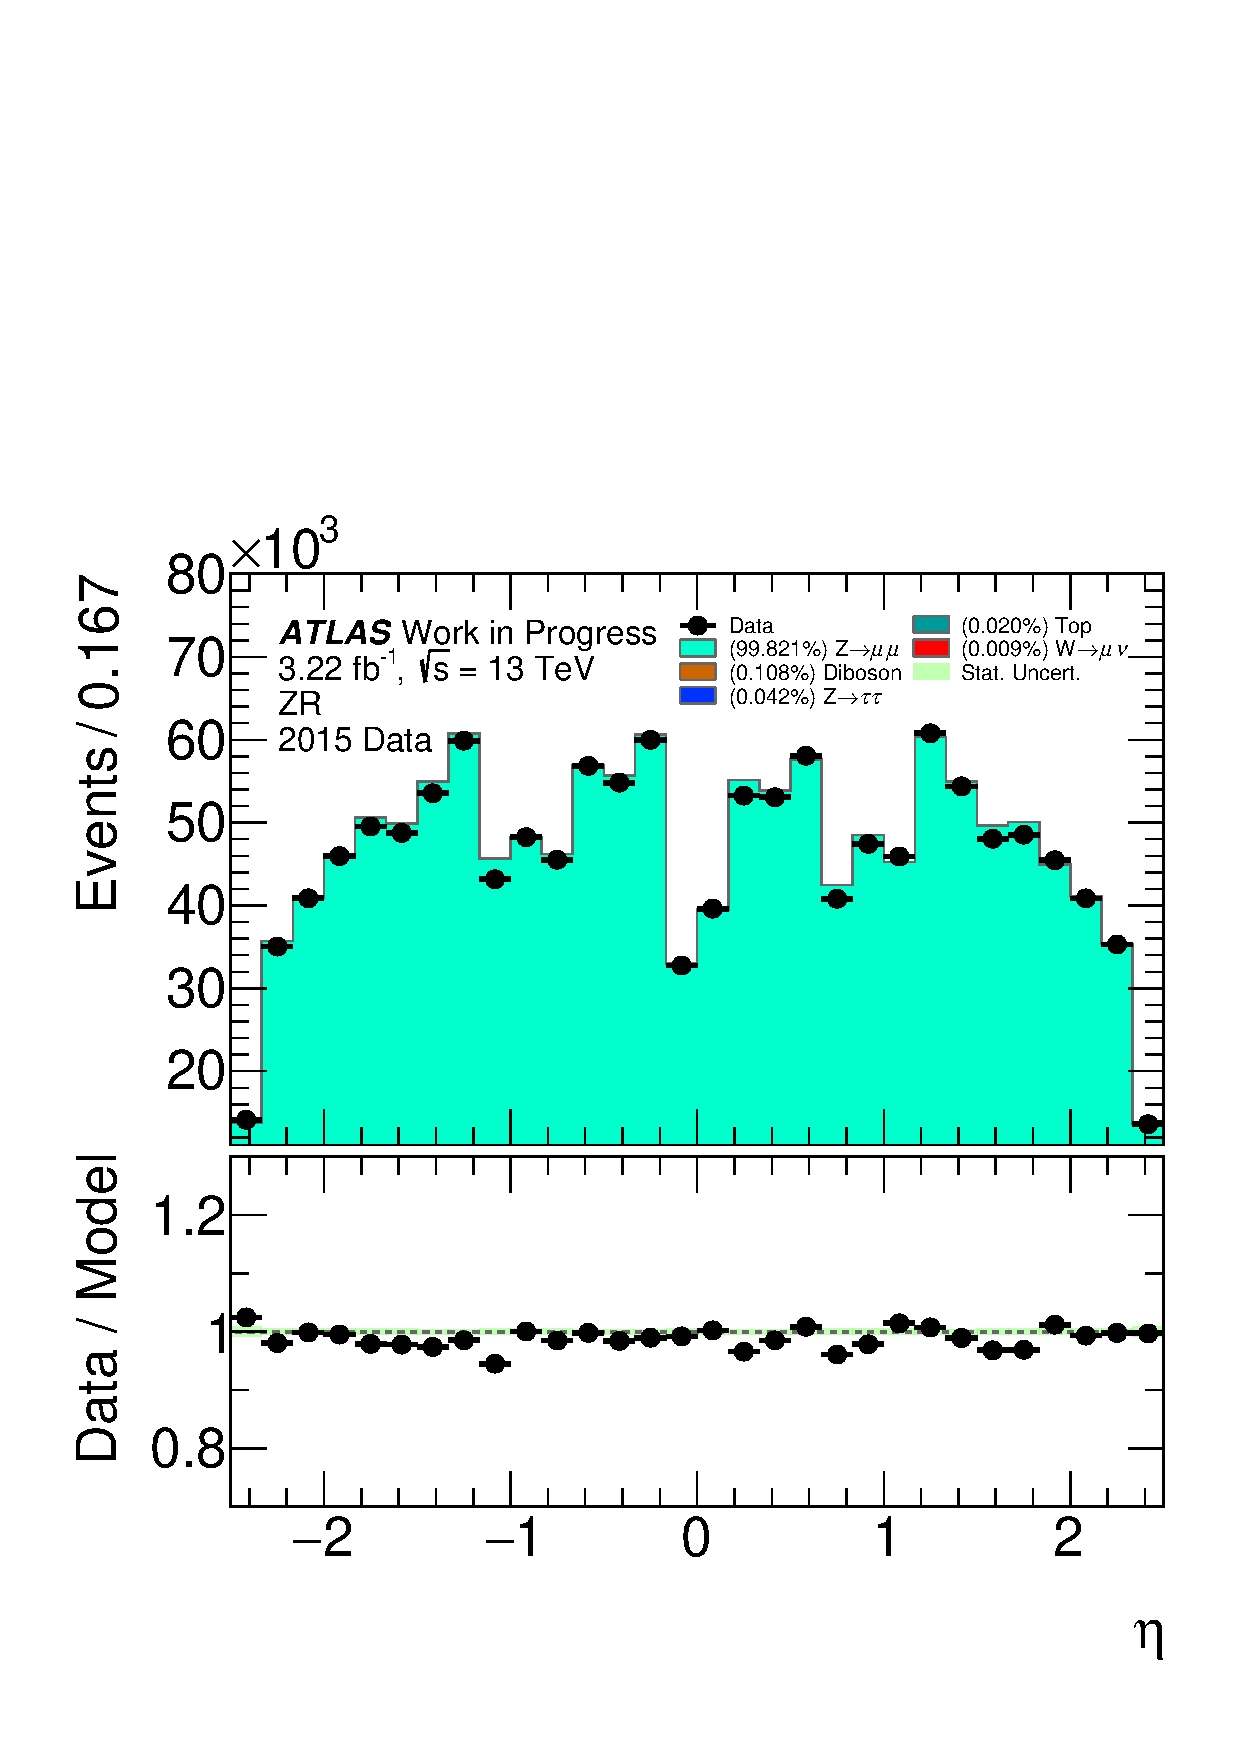
\includegraphics[width=0.45\textwidth]{figures/ZR/dataMc-lep_0_eta-ZR-mu.pdf}
\caption{
Leading lepton pseudorapidity distribution from the $Z \rightarrow e^+e^-$ selection (left) and the $Z \rightarrow \mu^+\mu^-$  selection (right).
The expected contributions from all backgrounds are estimated with Monte Carlo simulations.
The background processes are heavily suppressed and not visible on the linear scale. 
% Systematic uncertainties for the signal and background distributions are combined in the shaded band, and 
Statistical uncertainties are shown on the data points.
Luminosity uncertainties are not included.
}
\label{fig:ZR_lep_0_eta}
\end{figure}

\begin{figure}[htbp]
\centering
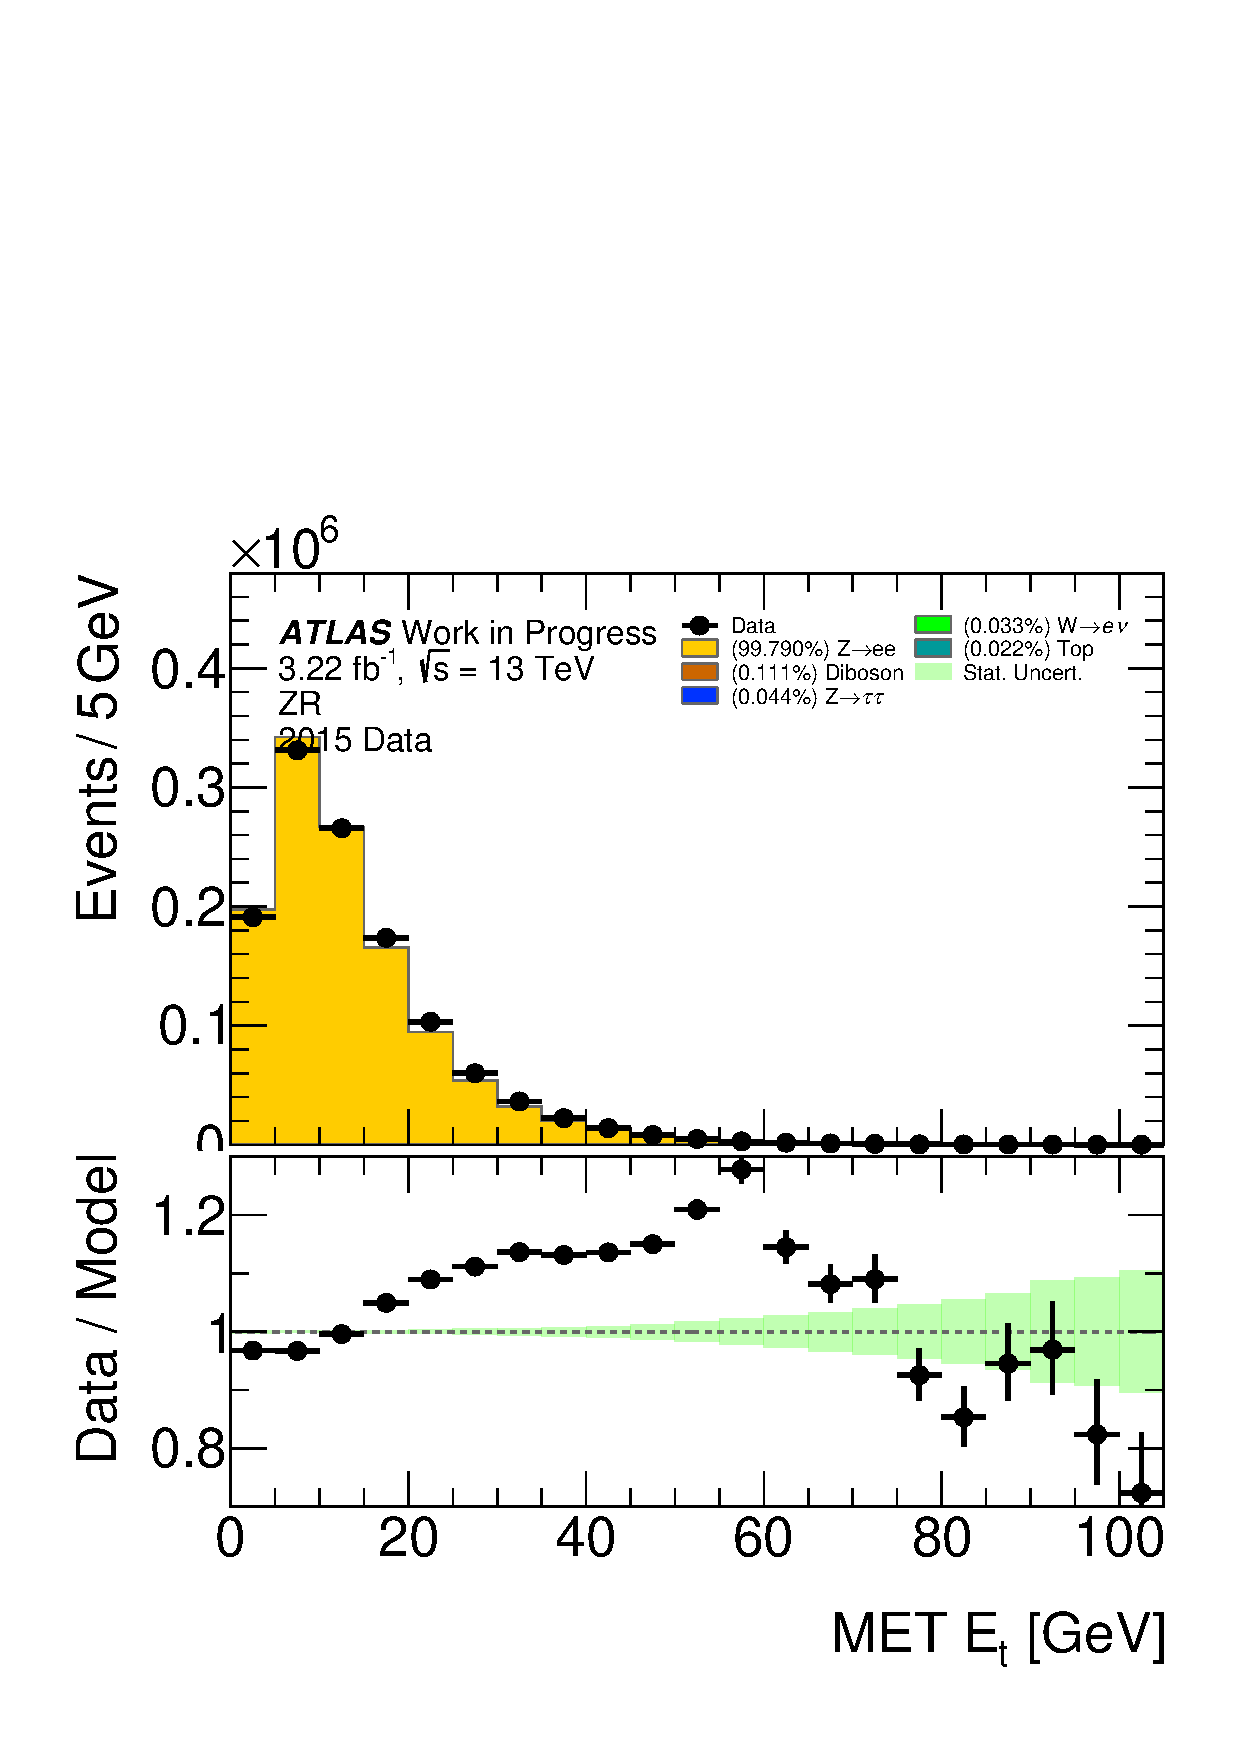
\includegraphics[width=0.45\textwidth]{figures/ZR/dataMc-met_reco_et-ZR-el.pdf}
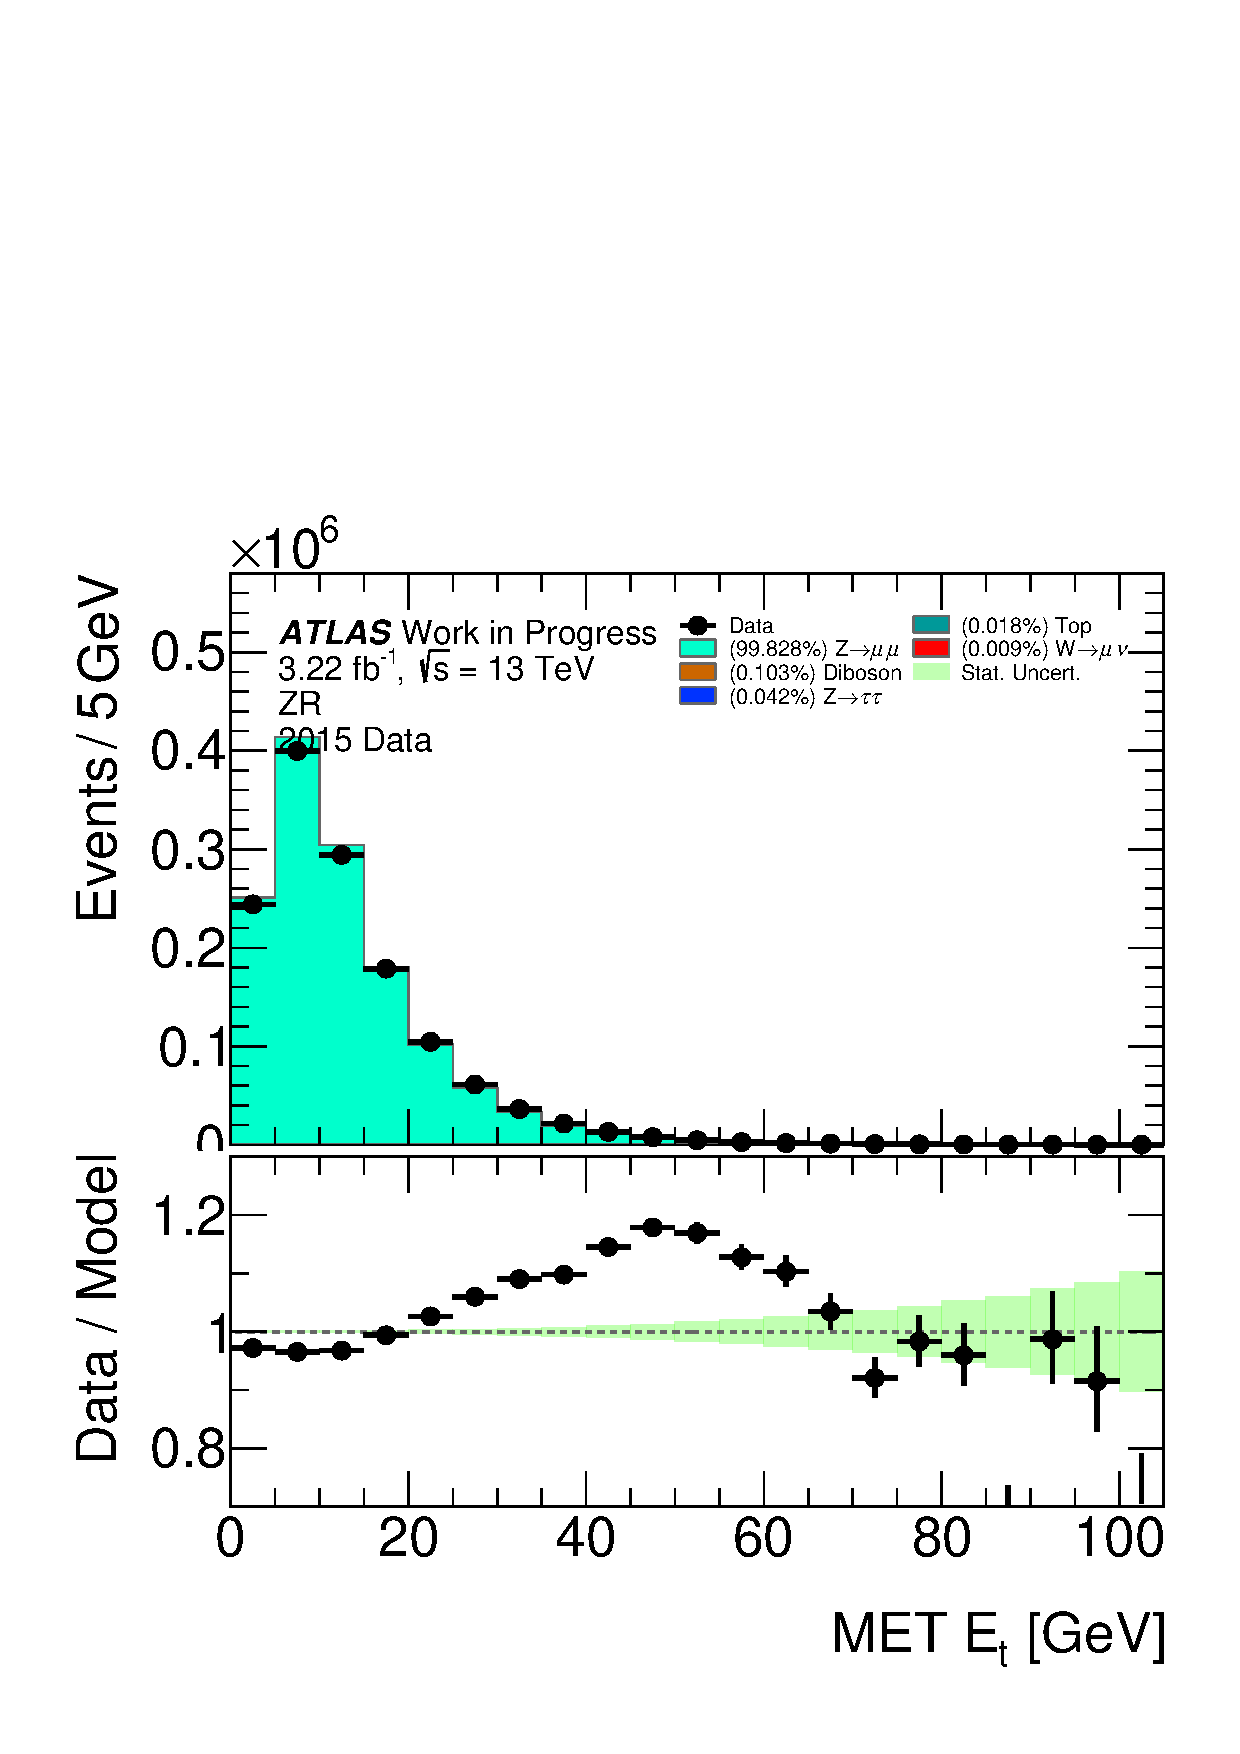
\includegraphics[width=0.45\textwidth]{figures/ZR/dataMc-met_reco_et-ZR-mu.pdf}
\caption{
 Missing transverse energy distribution from the $Z \rightarrow e^+e^-$ selection (left) and the $Z \rightarrow \mu^+\mu^-$  selection (right).
The expected contributions from all backgrounds are estimated with Monte Carlo simulations.
The background processes are heavily suppressed and not visible on the linear scale. 
% Systematic uncertainties for the signal and background distributions are combined in the shaded band, and 
Statistical uncertainties are shown on the data points.
Luminosity uncertainties are not included.
}
\label{fig:ZR_met_reco_et}
\end{figure}

\begin{figure}[htbp]
\centering
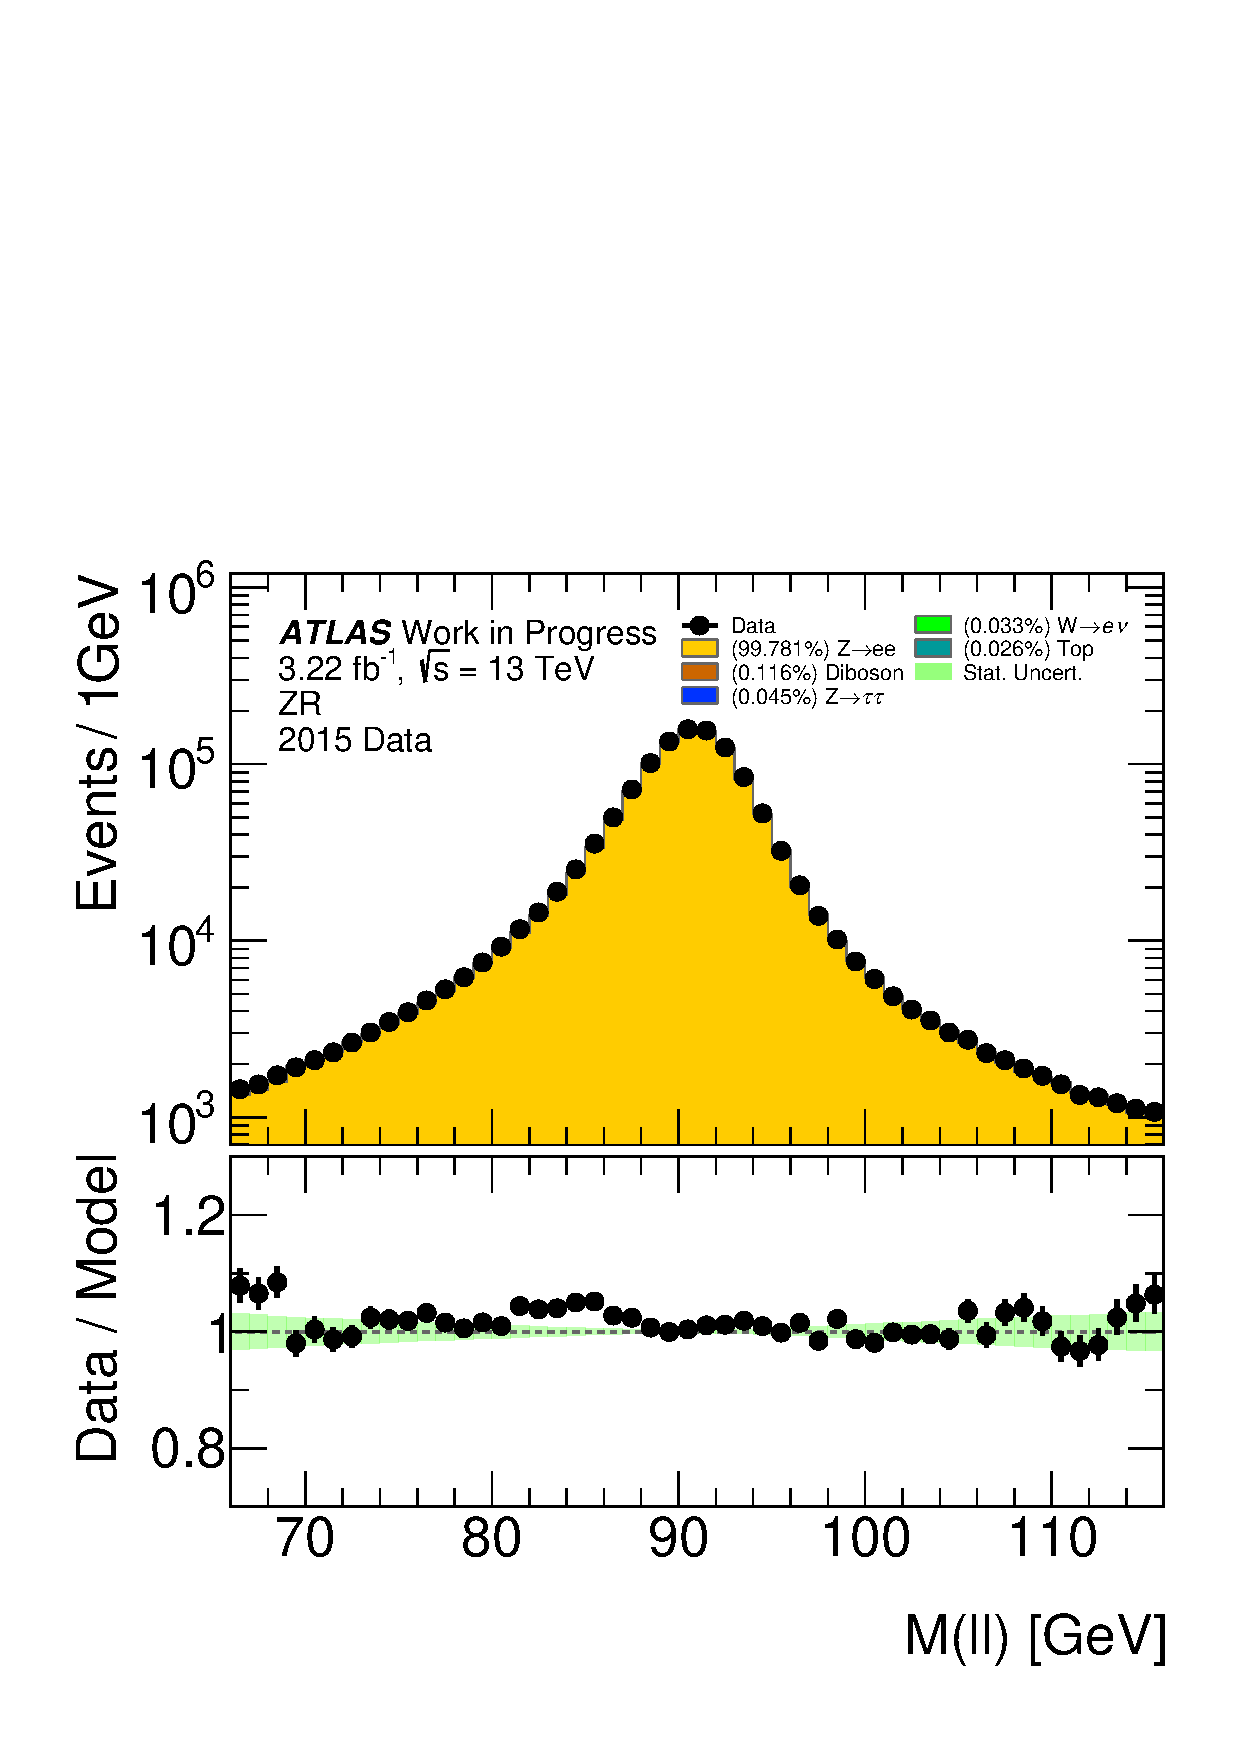
\includegraphics[width=0.45\textwidth]{figures/ZR/dataMc-dilep_m-ZR-el-log.pdf}
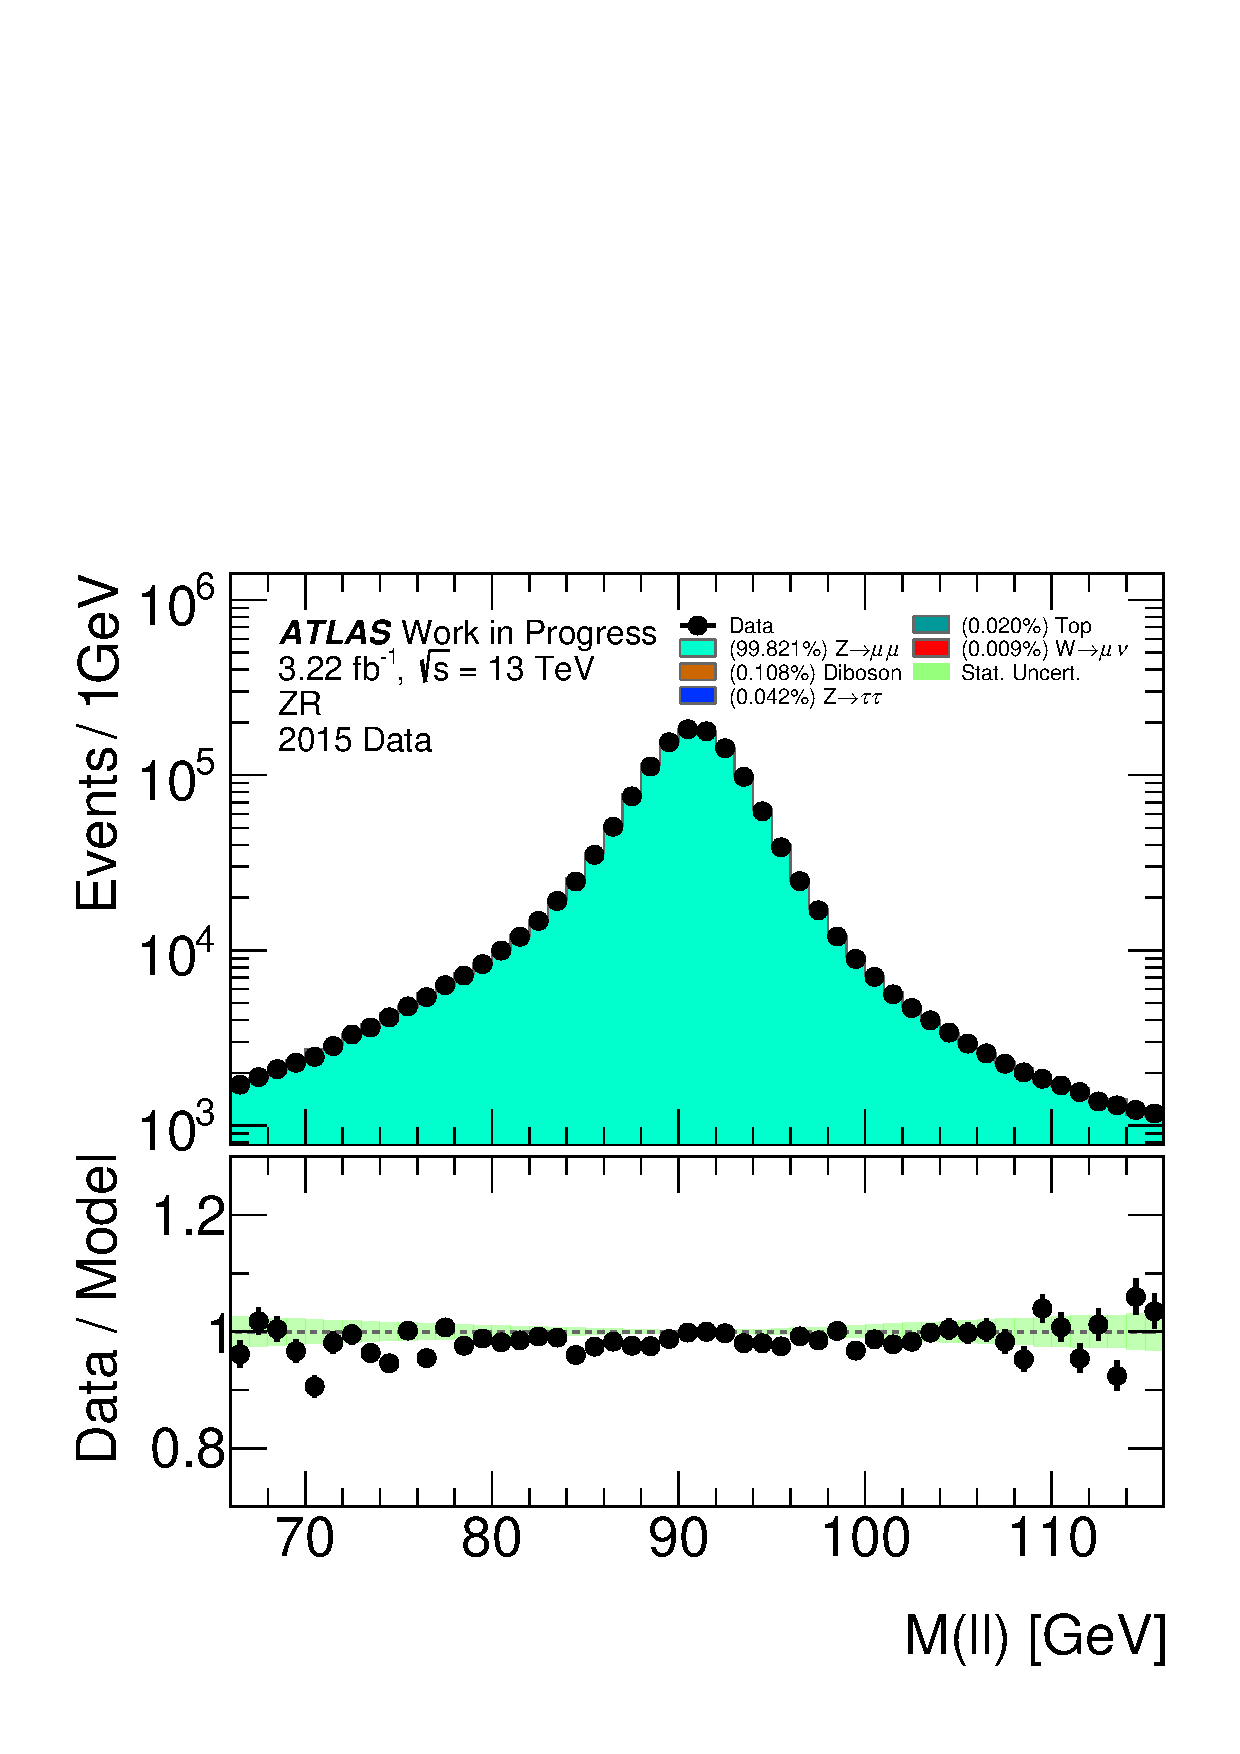
\includegraphics[width=0.45\textwidth]{figures/ZR/dataMc-dilep_m-ZR-mu-log.pdf}
\caption{
Dilepton mass distribution after the $Z \rightarrow e^+e^-$ selection (left) and the $Z \rightarrow \mu^+\mu^-$  selection (right).
Both leptons is required to satisfy $p_T > 27$ GeV.
The expected contributions from all backgrounds are estimated with Monte Carlo simulations.
% The background processes are heavily suppressed and not visible on the linear scale. 
% Systematic uncertainties for the signal and background distributions are combined in the shaded band, and 
Statistical uncertainties are shown on the data points.
Luminosity uncertainties are not included.
}
\label{fig:ZR_dilep_m_log}
\end{figure}

\begin{figure}[htbp]
\centering
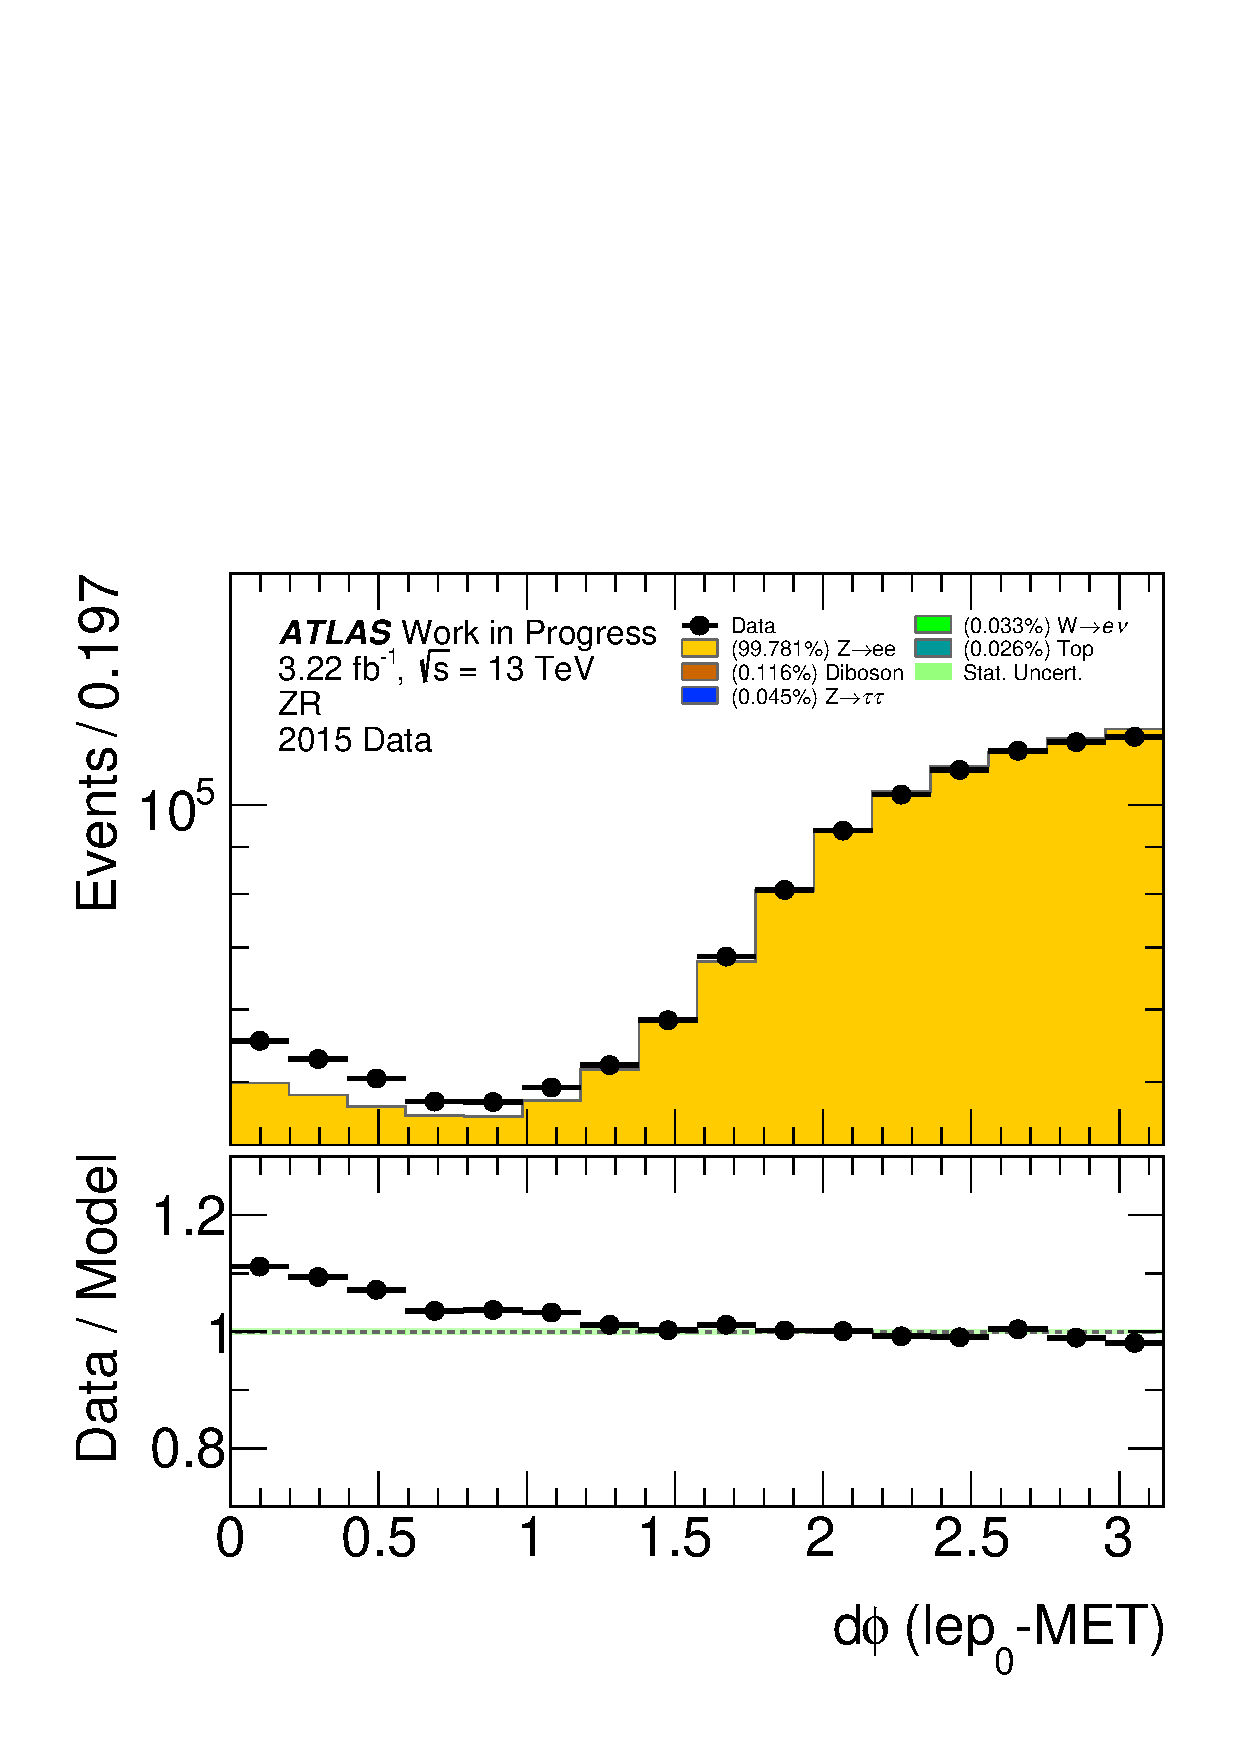
\includegraphics[width=0.45\textwidth]{figures/ZR/dataMc-lepmet_dphi-ZR-el-log.pdf}
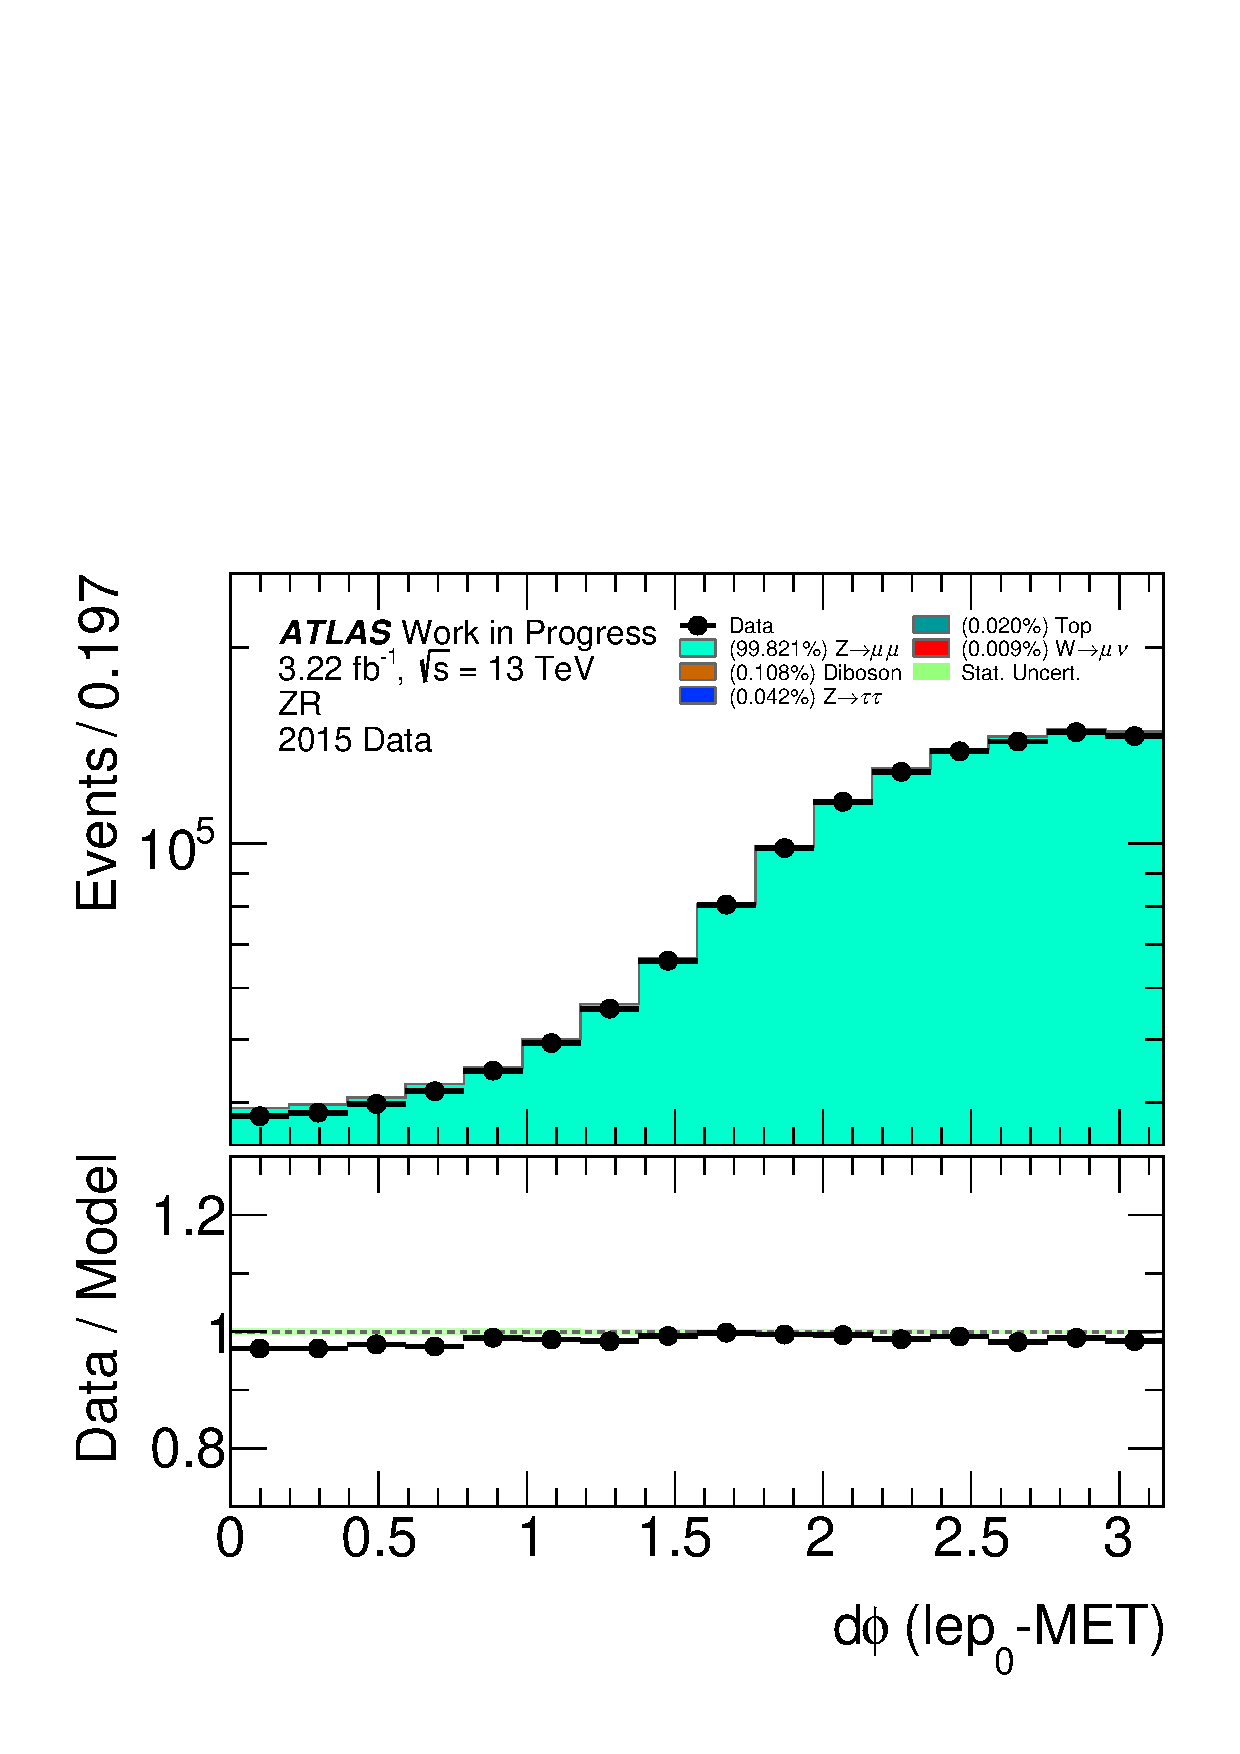
\includegraphics[width=0.45\textwidth]{figures/ZR/dataMc-lepmet_dphi-ZR-mu-log.pdf}
\caption{
Azimuthal angle distribution, calculated as azimuthal angle difference of the leading lepton and the $E_{T}^{miss}$ from the $Z \rightarrow e^+e^-$ selection (left) and the $Z \rightarrow \mu^+\mu^-$  selection (right).
The $E_{T}^{miss}$ has been recalibrated using the best energy calibration for each of the identified physics objects.
The expected contributions from all backgrounds are estimated with Monte Carlo simulations. 
% Systematic uncertainties for the signal and background distributions are combined in the shaded band, and 
Statistical uncertainties are shown on the data points.
Luminosity uncertainties are not included.
}
\label{fig:ZR_lepmet_dphi}
\end{figure}

\begin{figure}[htbp]
\centering
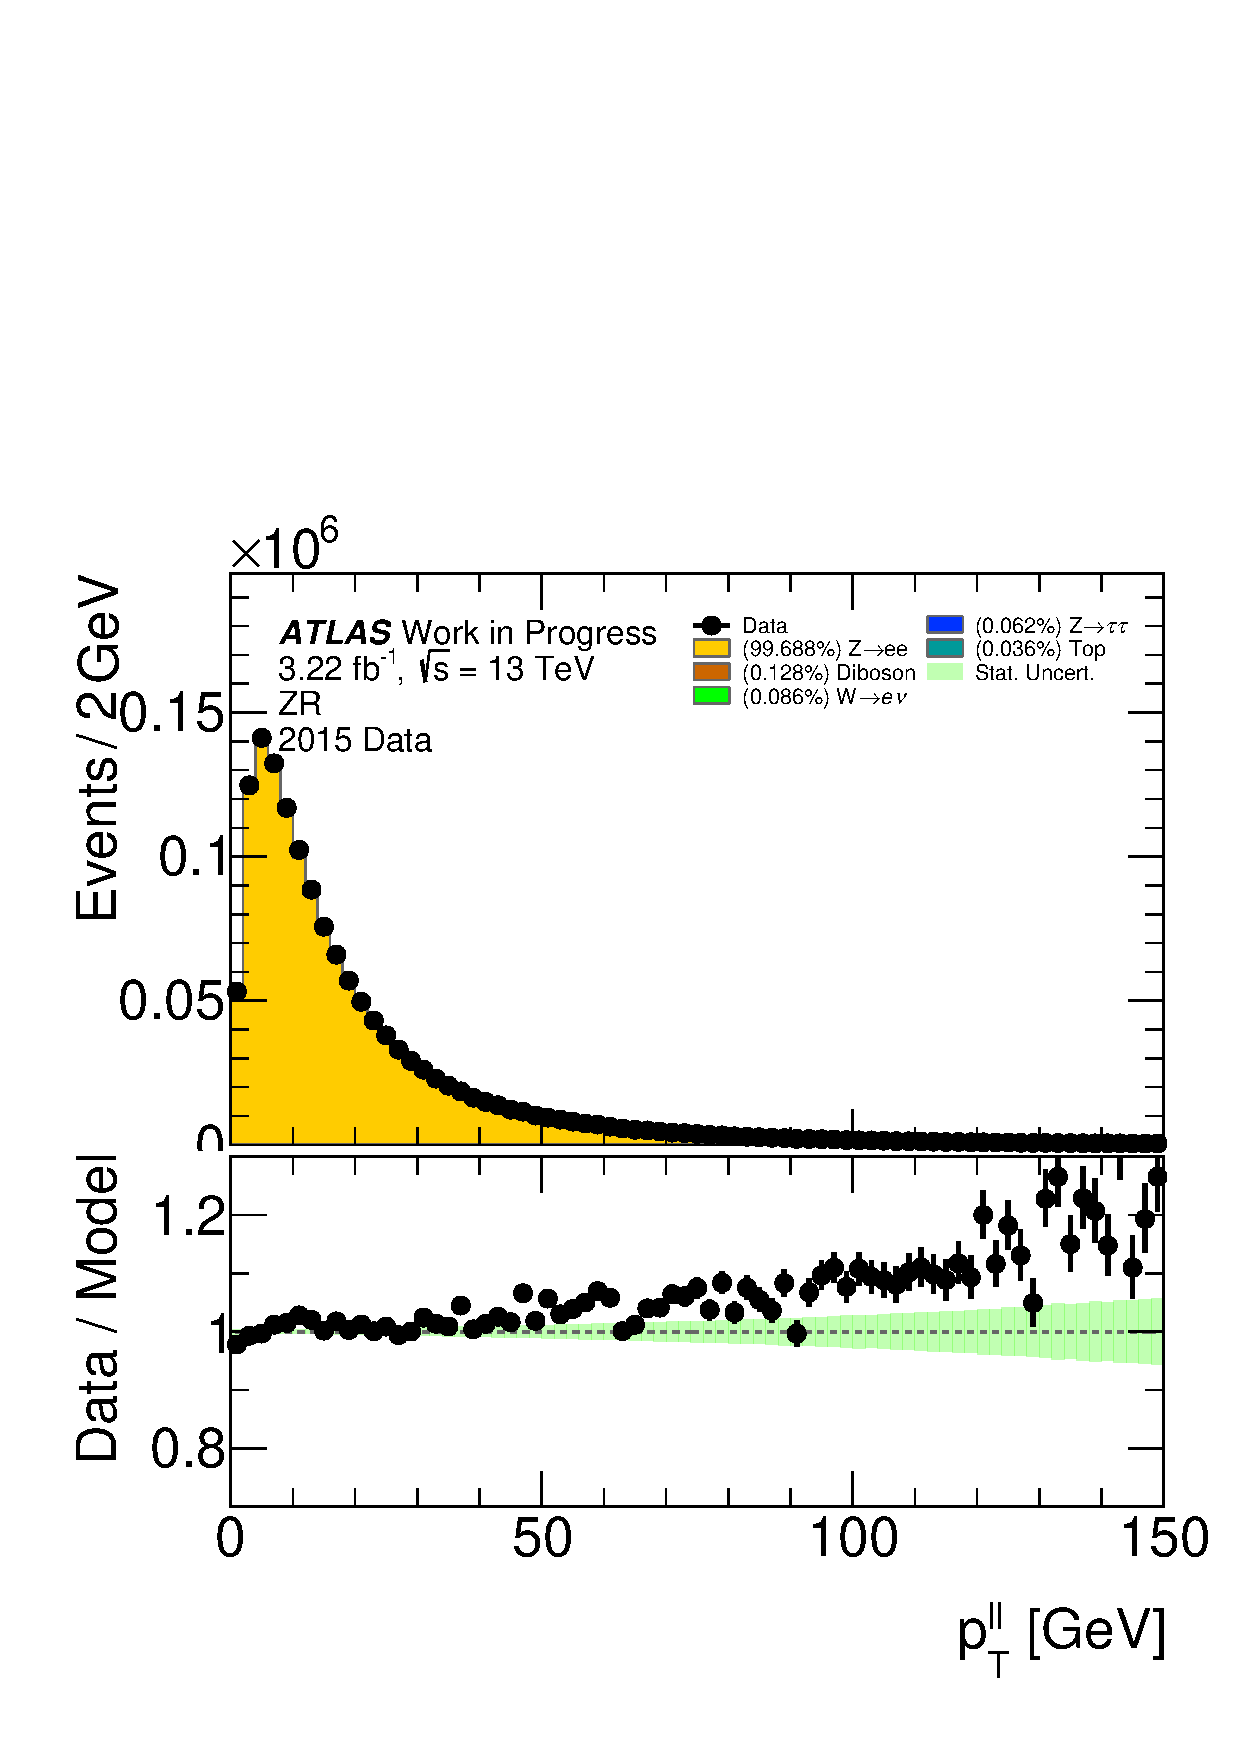
\includegraphics[width=0.45\textwidth]{figures/ZR/dataMc-dilep_pt-ZR-el.pdf}
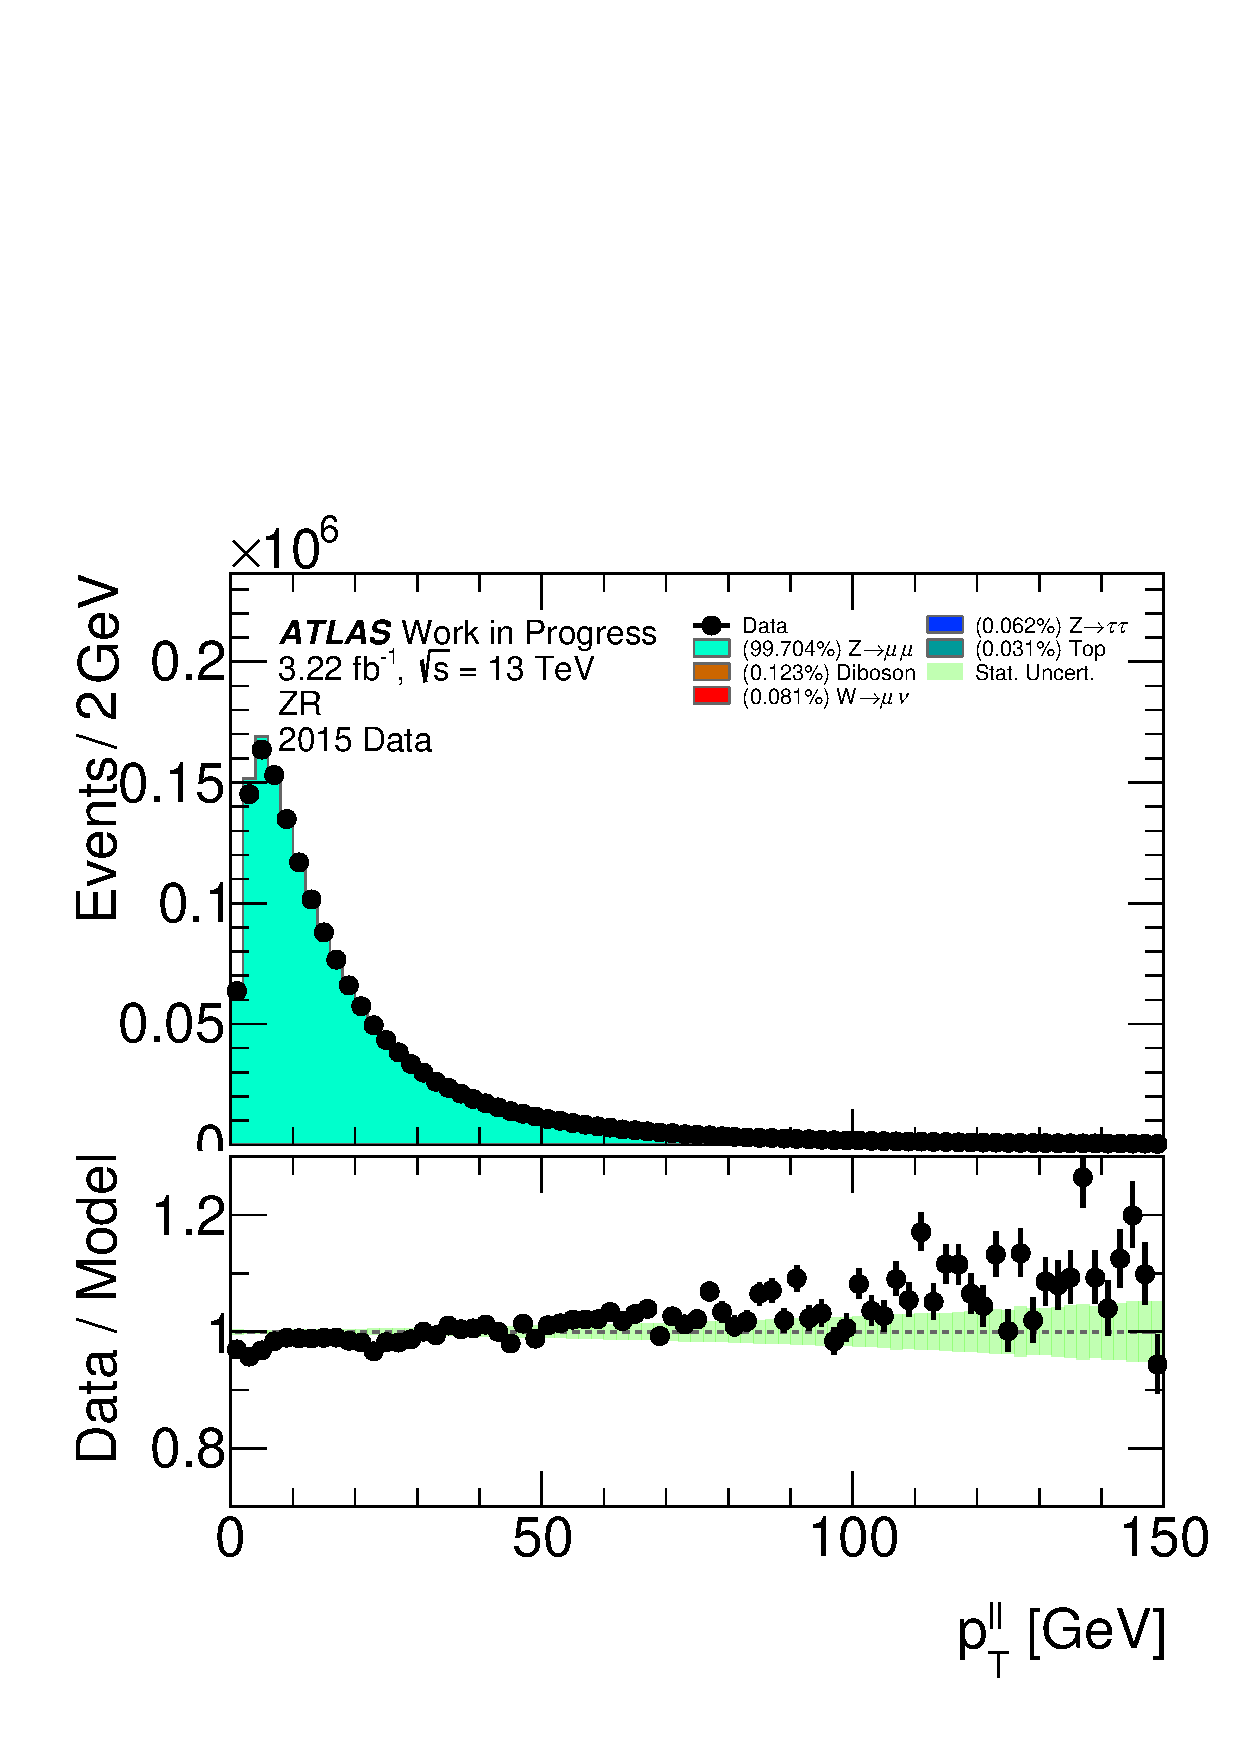
\includegraphics[width=0.45\textwidth]{figures/ZR/dataMc-dilep_pt-ZR-mu.pdf}
\caption{
Z boson transverse momentum distribution after the $Z \rightarrow e^+e^-$ selection (left) and the $Z \rightarrow \mu^+\mu^-$  selection (right).
The expected contributions from all backgrounds are estimated with Monte Carlo simulations.
The background processes are heavily suppressed and not visible on the linear scale. 
% Systematic uncertainties for the signal and background distributions are combined in the shaded band, and 
Statistical uncertainties are shown on the data points.
Luminosity uncertainties are not included.
}
\label{fig:ZR_dilep_pt}
\end{figure}

\begin{figure}[htbp]
\centering
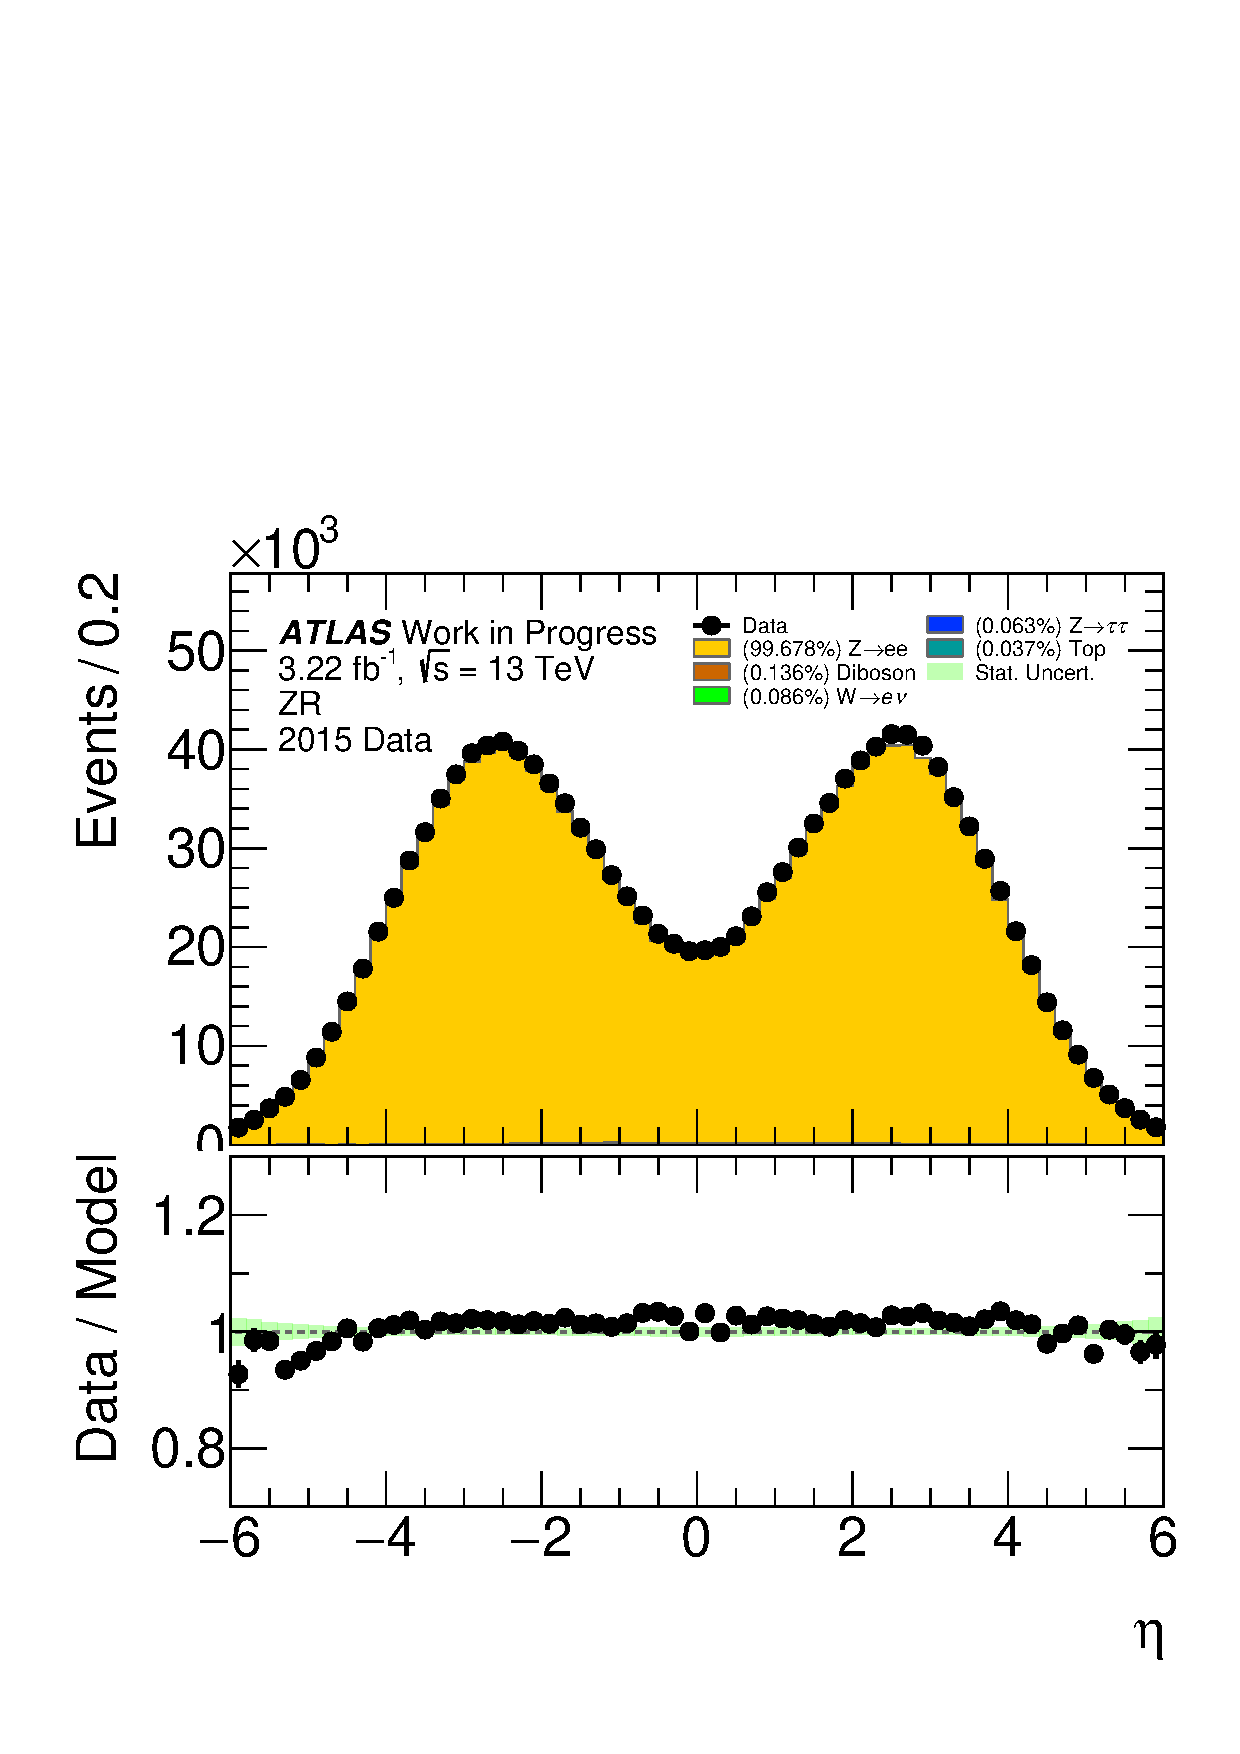
\includegraphics[width=0.45\textwidth]{figures/ZR/dataMc-dilep_eta-ZR-el.pdf}
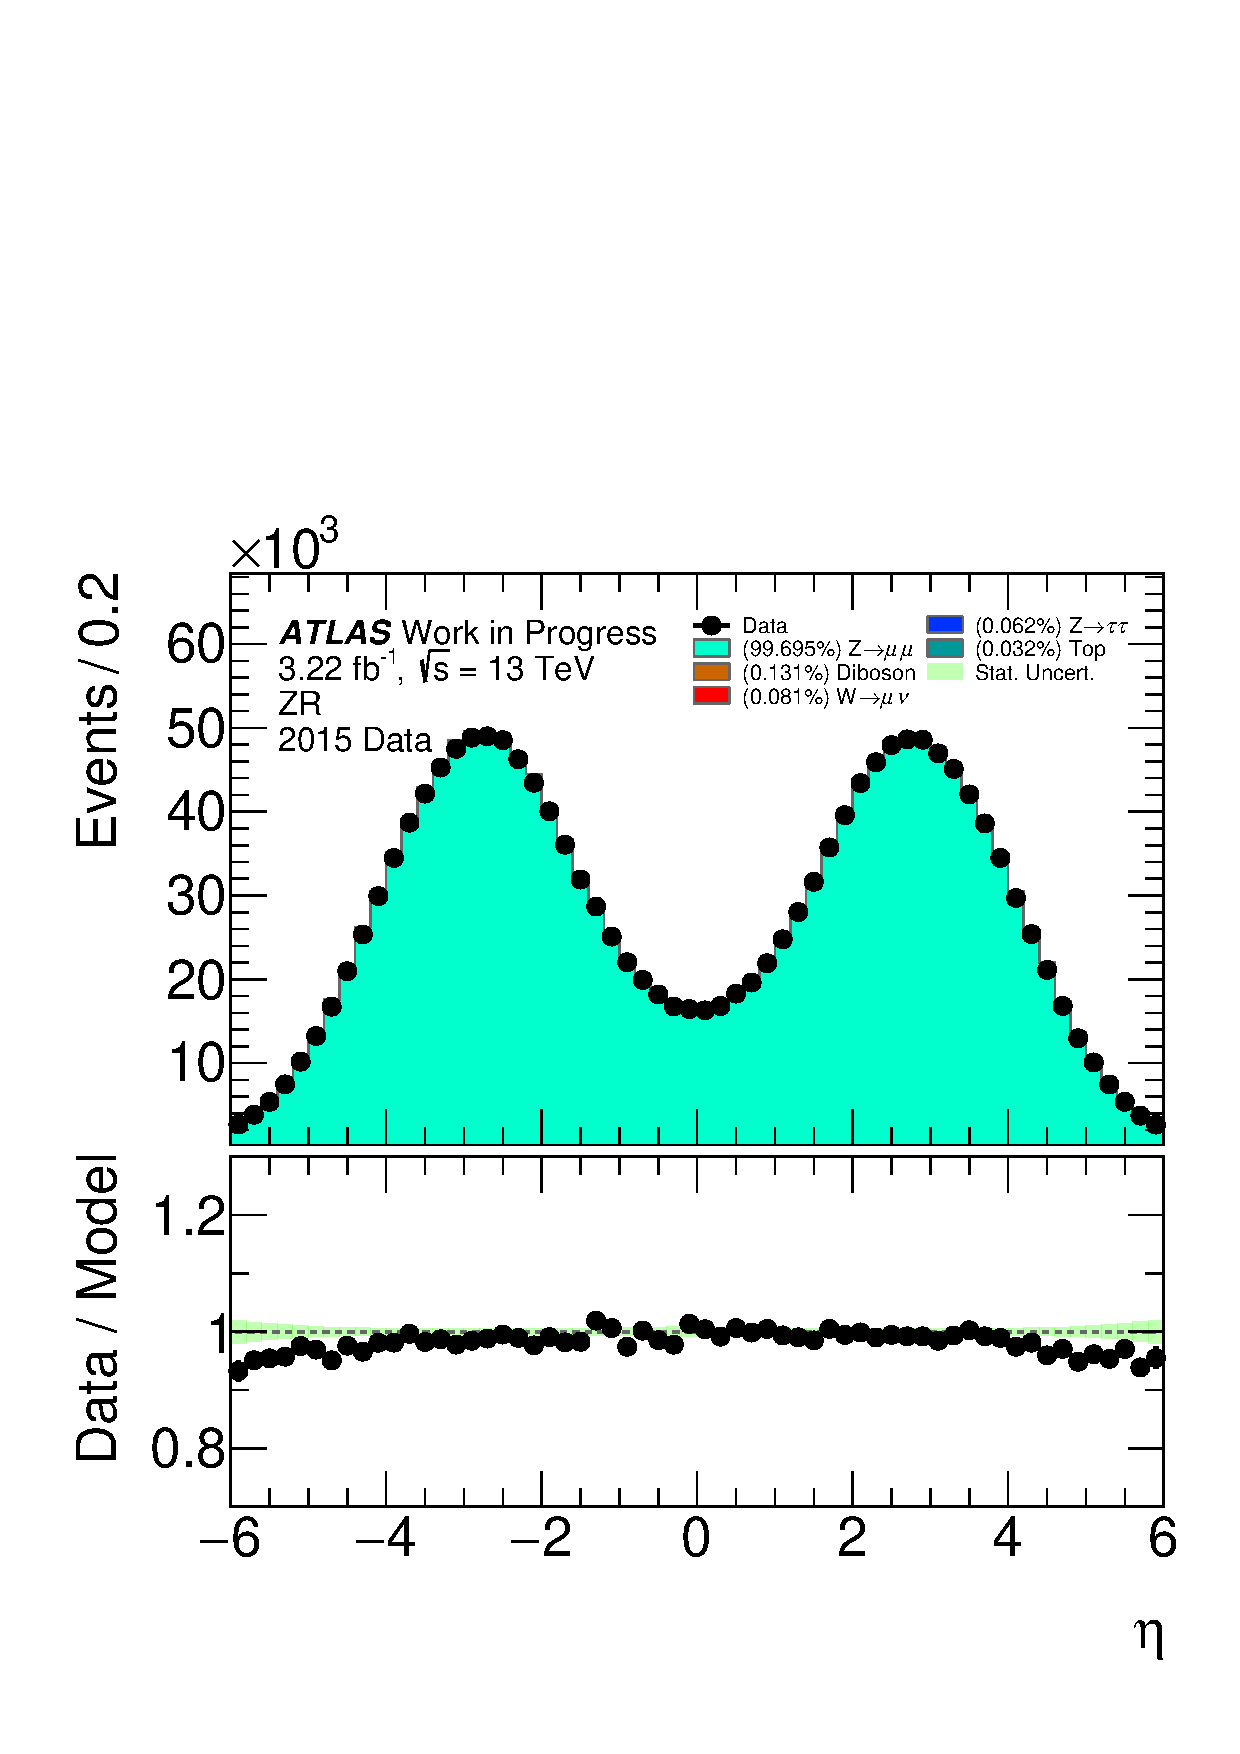
\includegraphics[width=0.45\textwidth]{figures/ZR/dataMc-dilep_eta-ZR-mu.pdf}
\caption{
Z boson pseudorapidity distribution after the $Z \rightarrow e^+e^-$ selection (left) and the $Z \rightarrow \mu^+\mu^-$  selection (right).
The expected contributions from all backgrounds are estimated with Monte Carlo simulations.
The background processes are heavily suppressed and not visible on the linear scale. 
% Systematic uncertainties for the signal and background distributions are combined in the shaded band, and 
Statistical uncertainties are shown on the data points.
Luminosity uncertainties are not included.
}
\label{fig:ZR_dilep_eta}
\end{figure}

\subsection{Background-subtracted W and Z candidate events}
\label{sec:Background_subtracted_candidate_events}

Tables~\ref{tbl:SR_observed_candidates} and~\ref{tbl:ZR_observed_candidates} summarise the numbers of observed candidate events for the $W \rightarrow \ell\nu$ and $Z \rightarrow \ell\ell$ channels, respectively, and include the number of expected background events from both the multijet process and electroweak plus $t\bar{t}$ processes and the number of background-subtracted signal events. 
The first uncertainty is due to statistics. 
% Monte Carlo statistical uncertainties are considered to be negligible in comparison to the statistical uncertainties associated to the data and to the estimation of the QCD background. 
\todo{The second uncertainty is a systematic one.}
The QCD background systematic uncertainties were explained in Section~\ref{sec:bkg_mj}. 
\todo{The luminosity determination uncertainty of 5\% is used.}

% ################################
% SR background composition table
% ################################

% \begin{table}[h]
% \begin{center}
%  \begin{tabular}{ | c || c || c | c || c |  } 
%  \hline
%  $\ell$ & Observed   &  Background & Background & Background-subtracted \\
%         & candidates & (EW + top)  & (Multijet) & Signal $N_{W\tau}^{sig}$ \\
%  \hline
%  \hline
%  $e^{\pm}$ &    &   &  & \\
%  \hline
%  $\mu^{\pm}$ &    &   &  & \\
%  \hline
% \end{tabular}
% \caption{
% Numbers of observed candidate events for the $W \rightarrow \tau\nu \rightarrow \ell\nu\nu$ channel, electroweak (EW) plus top, and data derived QCD background events, and background-subtracted signal events. 
% The first uncertainty is statistical.
% The second uncertainty represents the systematics (as described in the text).
% In addition to what is quoted in this table, \todo{an 5\%} uncertainty on the luminosity determination is applicable to the electroweak plus top background.
% The uncertainty considered for the EW+top backgrounds is the combination of the experimental uncertainties, described in \todo{Section 6}, the \todo{NNLO normalisation uncertainties}, described in \todo{Table 9}, and the statistical uncertainty on the MC.
% The uncertainty on the multijet estimate \todo{is shown as stat+syst}, as described in Section~\ref{sec:bkg_mj}.
% On $N - B$ the data statistical uncertainty, and the total systematic ones, obtained summing in quadrature the EW+top uncertainties, and the multijet statistical and systematic uncertainties.
% }
% \label{tbl:SR_observed_candidates}
% \end{center}
% \end{table}

\begin{table}[h]
\begin{center}
\begin{tabular}{ | c || c || c | c || c |  }
\hline
$\ell$ & Observed   &  Background & Background & Background-subtracted \\
        & candidates & (EW + top)  & (Multijet) & Signal $N_{W\tau}^{sig}$ \\
\hline
\hline
$e^{\pm}$ & 15844096.00 $\pm$ 3980.46 & 14448983.00 $\pm$ 11936.92 & 0.00 $\pm$ 0.00 & 1395113.00 $\pm$ 12583.09\\
\hline
$\mu^{\pm}$ & 16667946.00 $\pm$ 4082.64 & 16223126.65 $\pm$ 13865.15 & 0.00 $\pm$ 0.00 & 444819.35 $\pm$ 14453.73\\
\hline
\end{tabular}
\caption{
Numbers of observed candidate events for the $W \rightarrow \tau\nu \rightarrow \ell\nu\nu$ channel, electroweak (EW) plus top, and data derived QCD background events, and background-subtracted signal events.
The first uncertainty is statistical.
The second uncertainty represents the systematics (as described in the text).
% In addition to what is quoted in this table, \todo{an 5\%} uncertainty on the luminosity determination is applicable to the electroweak plus top background.
% The uncertainty considered for the EW+top backgrounds is the combination of the experimental uncertainties, described in \todo{Section 6}, the \todo{NNLO normalisation uncertainties}, described in \todo{Table 9}, and the statistical uncertainty on the MC.
The uncertainty on the multijet estimate \todo{is shown as stat+syst}, as described in Section~\ref{sec:bkg_mj}.
On $N - B$ the data statistical uncertainty, and the total systematic ones, obtained summing in quadrature the EW+top uncertainties, and the multijet statistical and systematic uncertainties.
}
\label{tbl:SR_observed_candidates}
\end{center}
\end{table}

% ################################
% ZR background composition table
% ################################

\begin{table}[h]
\begin{center}
\begin{tabular}{ | c || c || c || c |  }
\hline
$\ell$ & Observed   &  Background & Background-subtracted \\
        & candidates & (EW + top)  & Signal $N_{Z}^{sig}$ \\
\hline
\hline
$e^{\pm}$ & 1456927.00 $\pm$ 1207.03 & 4603.41 $\pm$ 120.20 & 1452323.59 $\pm$ 1213.00\\
\hline
$\mu^{\pm}$ & 1676489.00 $\pm$ 1294.79 & 5151.34 $\pm$ 139.06 & 1671337.66 $\pm$ 1302.24\\
\hline
\end{tabular}
\caption{
Numbers of observed candidate events for the $Z \rightarrow \ell\ell$ channel, electroweak (EW) plus top, and multijet background events, and background-subtracted signal events.
The first uncertainty is statistical.
The second uncertainty represents the systematics (as described in the text).
% In addition to what is quoted in this table, \todo{an 5\%} uncertainty on the luminosity determination is applicable to the electroweak plus top background.
The multijet background is estimated to have less than 0.1\% contribution and neglected.
}
\label{tbl:ZR_observed_candidates}
\end{center}
\end{table}

\clearpage